% A sample model to write a TFG project

% IMPORTANT!!! Substitute "draft" with "final" to render the final version of the TFG 
\documentclass[titlepage,openright,twoside,a4paper,final,12pt,spanish]{book}

% Configuring the environment to support spanish characters.
\usepackage[T1]{fontenc}
\usepackage[utf8]{inputenc}
\usepackage[spanish]{babel}
\selectlanguage{spanish}

\usepackage[pdftex,final]{graphicx}

% Style package
\usepackage{trinidad-TfG}
% Font Package (Palatino)
\usepackage{mathpazo}
\usepackage{tgpagella}
% Packages for specific capabilities
\usepackage{rotating} % for text rotation in tables
\usepackage{multirow} % for multirow in tables
\usepackage{subfigure} % Place subfigures in figure environment
% Packages for specific symbols
\usepackage{amssymb}
\usepackage{amsmath}
\usepackage{amsfonts}
\usepackage{eurosym} % Euro symbol
\usepackage{bbding} % for \XSolidBrush
\usepackage{pifont} % for \ding{55} (a check mark)
\usepackage{verbatim} % for comment environment
\usepackage{float}
\usepackage{microtype}
\usepackage{svg}
\usepackage{pdfpages}

\raggedbottom
\makeglossaries

\begin{document}

\author{Ismael Carrasco Mkhazni}{Grado en Ingeniería Informática - Ingeniería del Software}{D. }{15456902M}
\authorEMail{ismcarmkh@alum.us.es}
\authorURL{https://www.linkedin.com/in/ismael-carrasco-mkhazni-a06211167/}
\setTitle{King And Peasants}
%\setSubtitle{No subtitle}
\setUniversity{Universidad de Sevilla}
\copyrightText{Pon aquí cuestiones acerca del copyright}
\supervisor{Pablo Trinidad Martín-Arroyo}{Dr.~}{Lenguajes y Sistemas Informáticos}

\makeTitlePage

\pagestyle{empty}
\begin{dedication}
Tu dedicatoria aquí
\end{dedication}
\pagenumbering{roman}
\pagestyle{trinidadPhD}

\chapter*{Agradecimientos}

La culminación de este proyecto es el resultado no solo de nuestro esfuerzo conjunto, sino también del respaldo incondicional de quienes nos han rodeado durante estos meses de desarrollo.

Queremos expresar nuestra más sincera gratitud a nuestro tutor, por su inestimable guía académica, su rigor técnico y el tiempo dedicado a orientarnos. Sus consejos han sido clave para materializar este trabajo.

A nuestras familias, por ser nuestro pilar fundamental. Gracias por vuestra paciencia infinita, comprensión y por brindarnos siempre el entorno y la tranquilidad necesarios para superar los momentos de mayor exigencia.

Finalmente, a nuestros amigos, por su apoyo moral constante, por aligerar la carga de trabajo en los días más intensos y por celebrar con nosotros cada hito superado.

\input{resumen}
\chapter*{Abstract}
For many people born in the first decade of the 21st century, video games have established themselves as one of the main leisure activities, profoundly marking an entire generation. Digital entertainment has evolved across different platforms, from accessible browser games powered by \textit{Adobe Flash}, to major console productions and the closed ecosystems of mobile games. In this context, this Bachelor's Thesis, \textit{King and Peasant}, stems from an interest in video game architecture and the desire to invest academic effort into a creative and stimulating product. Furthermore, to overcome the typically isolated nature of university projects, it is proposed as a collaborative development between two individuals, simulating the dynamics and demands of a professional environment in the software industry. The central objective is the design, implementation, and deployment of the digital version of the asymmetric board game \textit{King and Peasant} on a multiplayer web platform, offering a persistent ecosystem utilizing modern technologies to ensure a seamless, synchronized, and highly available experience.

To achieve this goal, the strategic card game \textit{King and Peasant} has been adapted under the standards of an agile development cycle based on Scrum. This implementation was carried out using modern technologies such as React, Express, Node.js, MariaDB, and WebSockets, following the Model-View-Controller (MVC) architectural pattern. As a result, a functional and dockerized web application has been deployed, integrating a user management system, multiplayer waiting rooms (lobbies), and a real-time rules engine. This demonstrates that it is possible to use current web technologies to provide an interactive and smooth experience, supported by a solid and scalable technical foundation that meets the standards of professional software engineering.

\tableofcontents
\listoffigures
\listoftables
\newpage

\pagenumbering{arabic}
\newacronym{api}{API}{Application Programming Interface}
\newacronym{ci}{CI}{Continuous Integration}
\newacronym{cd}{CD}{Continuous Deployment}
\newacronym{dto}{DTO}{Data Transfer Object}
\newacronym{http}{HTTP}{Hypertext Transfer Protocol}
\newacronym{json}{JSON}{JavaScript Object Notation}
\newacronym{jwt}{JWT}{JSON Web Token}
\newacronym{mvc}{MVC}{Model-View-Controller}
\newacronym{orm}{ORM}{Object-Relational Mapping}
\newacronym{ui}{UI}{User Interface}
\newacronym{ux}{UX}{User Experience}
\newacronym{ws}{WS}{WebSockets}
\newacronym{dom}{DOM}{Document Object Model}
\newacronym{sql}{SQL}{Structured Query Language}
\newacronym{pve}{PvE}{Player vs Environment}
\newacronym{pvp}{PvP}{Player vs Player}
\newacronym{acid}{ACID}{Atomicity, Consistency, Isolation, Durability}
\newacronym{spa}{SPA}{Single Page Application}
\newacronym{edt}{EDT}{Estructura de Desglose del Trabajo}


\lineNumbersOn
\part{Introducción}
\input{Contexto}
\input{Objetivos}

\part{Organización del proyecto}
\chapter{Estado del Arte y Marco Tecnológico}

\begin{quotation}[Novelist]{Ernest Hemingway (1899--1961)}
The good parts of a book may be only something a writer is lucky enough to overhear or it may be the wreck of his whole damn life -- and one is as good as the other.
\end{quotation}

\begin{abstract}
En este capítulo presenta el estado del arte y el marco tecnológico que sustenta el desarrollo de \textit{King and Peasant}. En primer lugar, se analizan las soluciones existentes en la digitalización de juegos de mesa, justificando la adopción de un modelo basado en la automatización de reglas frente a la simulación física. A continuación, se detalla y justifica la elección del \textit{stack} tecnológico, abordando la arquitectura de comunicación mediante \textit{WebSockets}, el entorno de ejecución asíncrono en \textit{Node.js}, el renderizado reactivo con \textit{React} y un sistema de persistencia dual basado en \textit{MariaDB} y \textit{Redis}. Finalmente, se expone la estrategia de contenedorización con \textit{Docker} y la política de pruebas automatizadas para garantizar la calidad y portabilidad del sistema.
\end{abstract}

\section{Análisis de soluciones existentes y estado del arte}

En la actualidad existen dos acercamientos a la hora de digitalizar un juego de mesa contemporáneo como lo es \textit{King and Peasant}. Por un lado, tenemos el ejemplo de \textit{Tabletop Simulator} (véase la Figura \ref{fig:tabletop}), que se basa en un entorno de simulación física operando como un "cajón de arena" (\textit{sandbox}) \cite{woods_eurogames}. El cumplimiento de las reglas se delega íntegramente a los usuarios, careciendo de una validación lógica que incrementa la carga cognitiva del usuario y ralentiza el flujo de la partida.

Por otro lado, se encuentra \textit{Board Game Arena} (véase la Figura \ref{fig:bga}), que está basado en un motor de validación de estados. En este modelo el cumplimiento de las reglas y las transiciones de estado se delegan al sistema, actuando así como un árbitro imparcial dentro de la partida garantizando la integridad de las mecánicas \cite{elias_characteristics}. El presente TFG se alinea con este segundo enfoque, ya que lo que se busca es crear un motor de reglas estricto que ofrezca una experiencia de juego automatizada, accesible desde el navegador y libre de la fricción que suponen los simuladores tridimensionales

\begin{figure}[H]
    \centering
    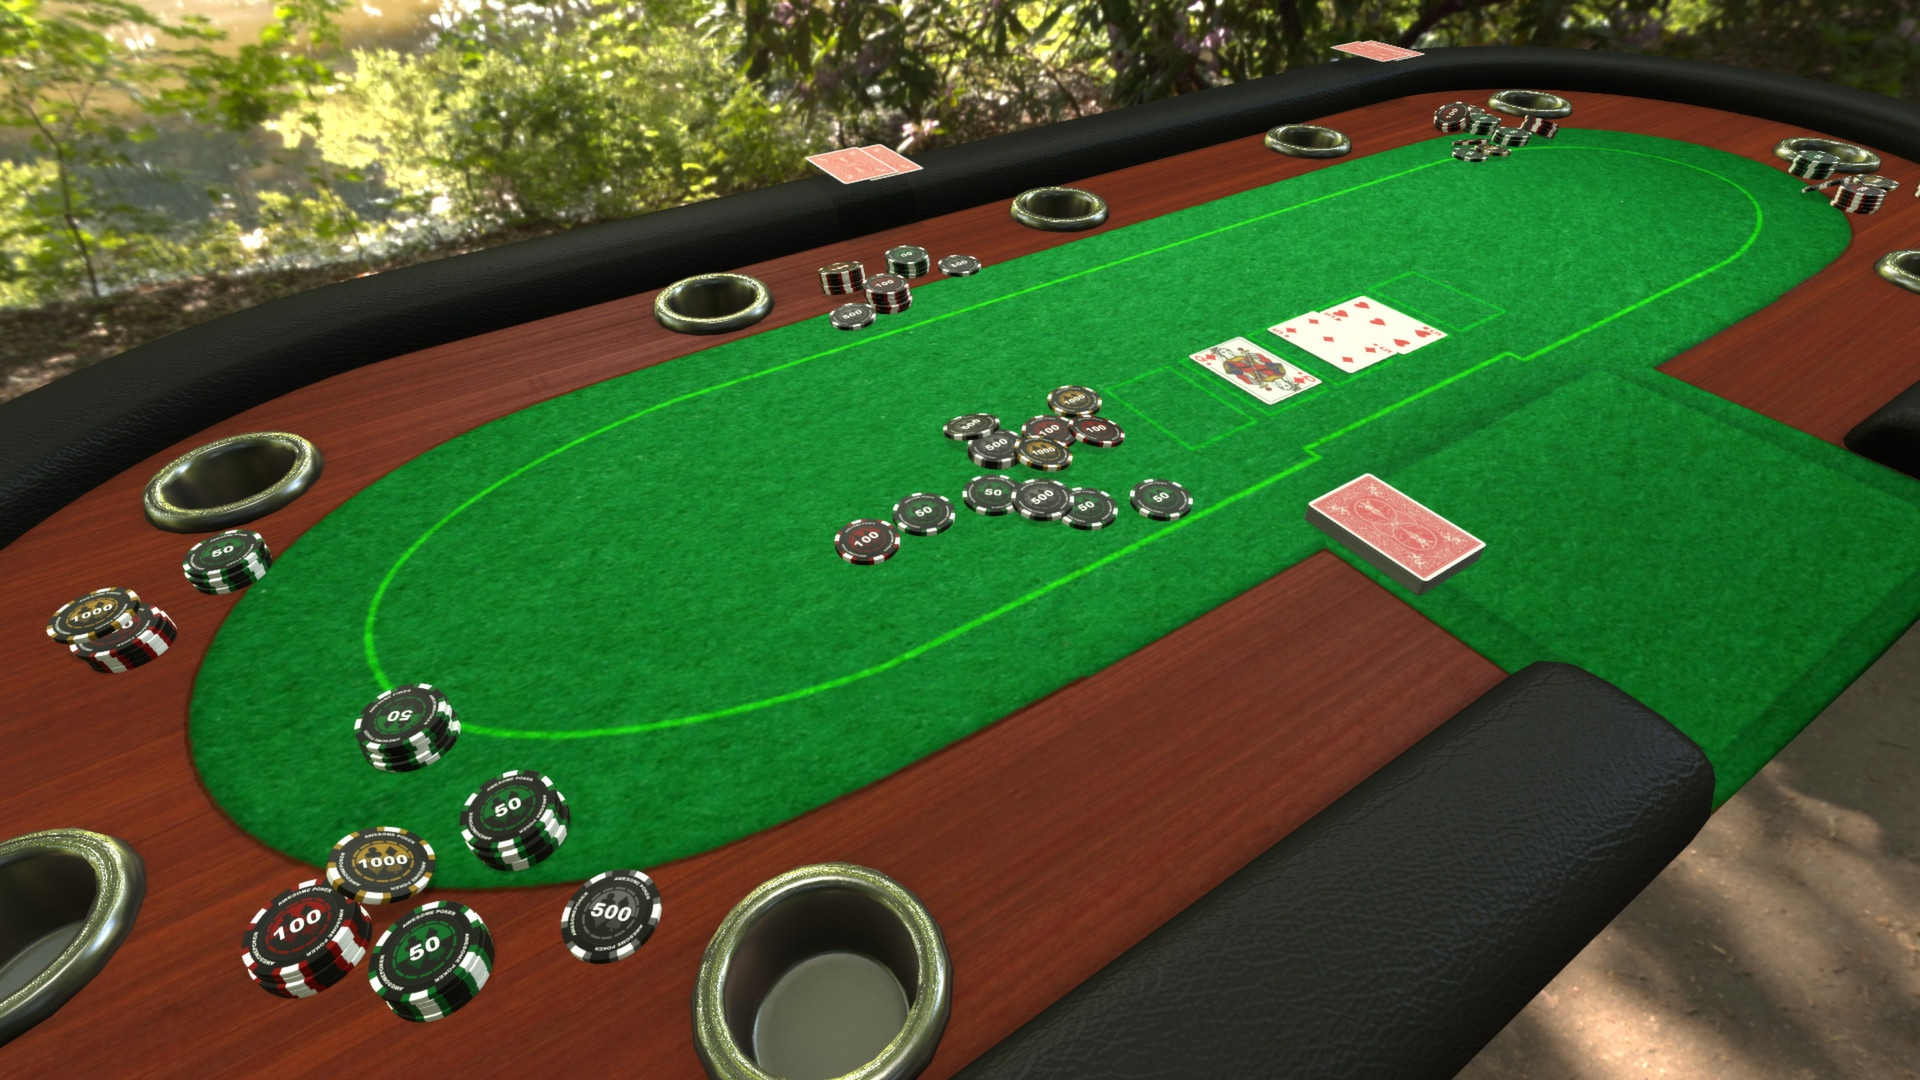
\includegraphics[width=0.8\textwidth]{figures/tabletop-cover_yezh.jpg}
    \caption{Interfaz de \textit{Tabletop Simulator}, basada en la simulación física tridimensional sin validación de reglas.}
    \label{fig:tabletop}
\end{figure}

\begin{figure}[H]
    \centering
    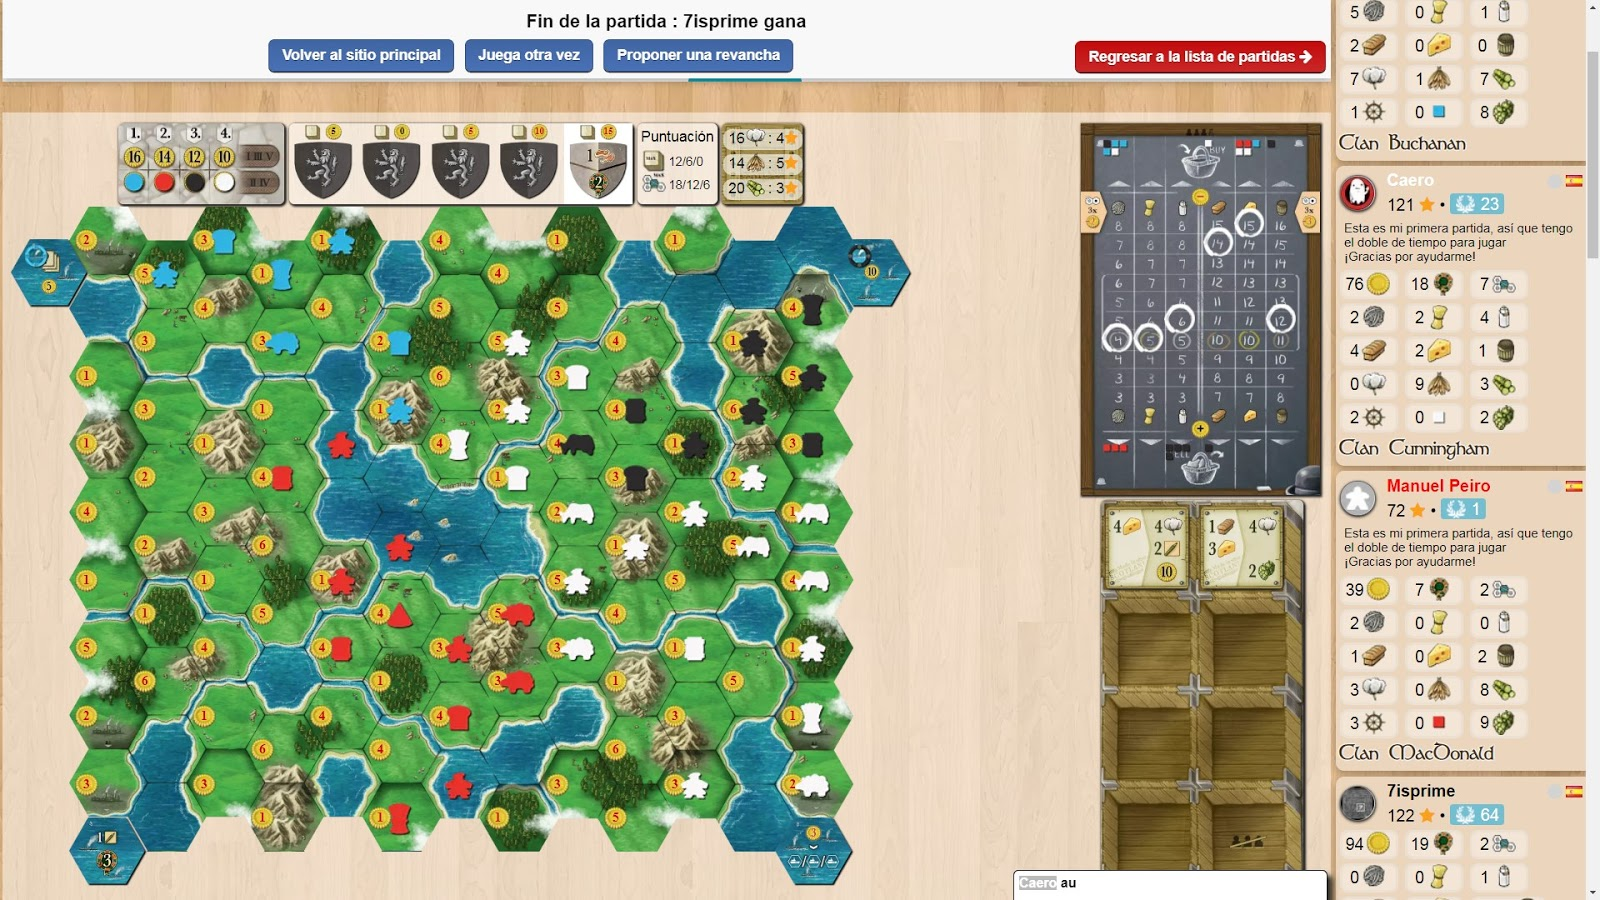
\includegraphics[width=0.8\textwidth]{figures/caledoniaBGALR.jpg}
    \caption{Interfaz de \textit{Board Game Arena}, basada en la automatización del estado de la partida en 2D.}
    \label{fig:bga}
\end{figure}

\section{Arquitectura de comunicación y sincronización}

Dada la naturaleza interactiva de un juego multijugador, la sincronización en tiempo real entre múltiples clientes es un punto crítico dentro del desarrollo de \textit{King and Peasant}. Para este propósito, implementar el motor del juego sobre una arquitectura web tradicional resultaba inviable debido a las limitaciones estructurales del protocolo \textit{HTTP}. El uso de técnicas como el \textit{Long-Polling} (\textit{polling}), donde el cliente interroga constantemente al servidor en busca de actualizaciones, introduciría una sobrecarga significativa en la red debido al envío repetitivo de cabeceras HTTP, generando latencias perceptibles que degradan la experiencia de juego \cite{rfc6202}.

Como alternativa a una API REST, se decidió utilizar el protocolo \textit{WebSocket} como núcleo de las comunicaciones de la partida. Como define el estándar oficial de la IETF \cite{rfc6455}, esta tecnología proporciona un canal de comunicación bidireccional sobre una única conexión TCP persistente. Esto permite el envío de eventos asíncronos (\textit{server-push}) en el mismo instante en el que se modifica el estado, validando las jugadas y actualizando instantáneamente la interfaz de todos los clientes conectados, reduciendo a su vez el coste computacional y garantizando una sincronización  fluida.

\section{Tecnologías de \textit{Backend} y Ecosistema de Desarrollo}

El alto volumen de conexiones concurrentes que presenta un juego multijugador exige un entorno de ejecución capaz de gestionar con eficiencia el consumo elevado de recursos que se produce al mantener las conexiones abiertas en un estado de sincronización permanente. En el caso de los servidores web tradicionales, el modelo de concurrencia basado en hilos (\textit{thread-per-request}) se ve afectado por el cambio de contexto (\textit{context switching}) \cite{tilkov_node}, provocando un rápido agotamiento de la memoria y cuellos de botella. Por otro lado, la mantenibilidad del código y el uso de lenguajes unificados constituyó un factor determinante a la hora de decantarse por una arquitectura de servidor. 

Por estos motivos, se adoptó \textit{Node.js}. Su arquitectura basada en un bucle de eventos (\textit{Event Loop}) procesa las solicitudes de red de forma asíncrona, evitando bloquear el hilo principal durante la espera de respuestas de la base de datos o de los clientes. Este diseño arquitectónico permite al sistema mantener activas miles de conexiones bidireccionales de manera simultánea con un consumo residual de recursos. Además, la capacidad de usar lenguajes isomórficos reduce la sobrecarga cognitiva del equipo de desarrollo y permite la compartición directa de módulos lógicos entre cliente y servidor \cite{cantelon_node}.

\section{Tecnologías de Frontend Reactividad de Interfaz}

La implementación de un juego de mesa en un entorno digital multijugador requiere elementos como un tablero interactivo, el cual, en términos de ingeniería, no es más que la proyección visual de una compleja máquina de estados. Sin embargo, se plantea una serie de retos técnicos a la hora de diseñar este componente. 

En primer lugar, la manipulación directa del \textit{Document Object Model} (DOM) para actualizar la interfaz resulta computacionalmente ineficiente. El navegador se ve obligado a recalcular estilos y repintar la pantalla cada vez que se produce una modificación, lo que provoca que la fluidez de la experiencia se vea degradada \cite{mardan_react}. En segundo lugar, abordar una interfaz que cuenta con tableros, mazos, perfiles y salas de espera bajo una arquitectura monolítica dificultaría enormemente su mantenibilidad y fomentaría la duplicación de código. Finalmente, se le suma el riesgo de desincronización de los estados visuales, resultando en validaciones del \textit{backend} que no se reflejan en la información gráfica \cite{banks_react}.  

Como solución a todos estos problemas, la arquitectura del cliente se construyó utilizando \textit{React}, una librería que impone un paradigma de desarrollo declarativo y basado en componentes. En primer lugar, gracias a la implementación de un \textit{Virtual DOM}, la ineficiencia computacional se mitiga. Al recibir un nuevo evento, \textit{React} genera una representación en memoria de la interfaz y la compara con la actual mediante un algoritmo de diferenciación (\textit{diffing}), aplicando al DOM real únicamente las modificaciones estrictamente necesarias. En segundo lugar, su arquitectura modular minimiza el riesgo que supone construir un sistema monolítico, permitiendo dividir la interfaz en unidades lógicas aisladas e independientes, facilitando la encapsulación y garantizando la mantenibilidad a largo plazo del código. Por último, el paradigma declarativo de \textit{React} permite concibir la interfaz matemáticamente como una función del estado subyacente ($UI = f(estado)$) \cite{banks_react}, convirtiendo el tablero en un reflejo exacto de la información de la partida y las reglas dictaminadas por el \textit{backend} \cite{mardan_react}.

\section{Gestión de la persistencia de datos}

Dentro de la información gestionada por el ecosistema encontramos requisitos técnicos independientes, lo que implica la necesidad de implementar un enfoque de persistencia adecuado para cada uno de ellos fundamentado en su naturaleza. Por un lado, la información estructural, como pueden ser las credenciales, perfiles de usuario, historial de partidas o la gestión de salas de espera (\textit{lobbies}), exige un almacenamiento persistente y estructurado que garantice las propiedades ACID (Atomicidad, Consistencia, Aislamiento y Durabilidad) \cite{elmasri_db}. Para satisfacer esta necesidad, y tras evaluar alternativas relacionales robustas como \textit{PostgreSQL}, se seleccionó el motor de bases de datos relacional \textit{MariaDB} por su agilidad en consultas y su perfecta integración con el ecosistema de \textit{Node.js}. Este motor se encarga de gestionar de forma centralizada la información de los usuarios y la configuración inicial de las partidas. La interacción con este motor relacional se abstrajo mediante \textit{Prisma ORM}, una decisión que previene vulnerabilidades de inyección SQL y garantiza un tipado estricto entre el esquema de la base de datos y la lógica del \textit{backend}.

Por otro lado, el estado del tablero interactivo se convierte en un dato efímero sometido a un volumen masivo de operaciones de lectura y escritura concurrentes. Hacer uso de una base de datos relacional para registrar las modificaciones generaría un cuello de botella debido a la latencia de entrada/salida (I/O), ralentizando la comunicación. Para mitigar este problema, se implementó \textit{Redis} como almacén de estructuras de datos en memoria (\textit{In-Memory Data Grid}) \cite{carlson_redis}. A diferencia de sistemas de caché simples como \textit{Memcached}, \textit{Redis} soporta el manejo nativo de estructuras de datos complejas, una característica indispensable para modelar el estado de un juego. Hacer uso de la memoria RAM para almacenar el estado dinámico de la partida permite que el servidor valide y comparta el resultado de las jugadas con tiempos de respuesta mucho menores, delegando en \textit{MariaDB} la persistencia del resultado final una vez concluido el encuentro.

\section{Contenedorización y automatización de pruebas}

El complejo funcionamiento intrínsico del motor de reglas asimétrico requería mecanismos rigurosos para garantizar la calidad y la estabilidad del software. El mal funcionamiento de las validaciones de estado o de las transiciones de la partida degradaría la experiencia de juego. En respuesta, haciendo uso de los marcos de trabajo \textit{Jest} y \textit{Vitest}, se implementó una batería de pruebas automatizadas que aseguraban el correcto comportamiento del motor de validación ante cualquier escenario \cite{myers_testing}. Dichas herramientas han permitido aislar y testear unitariamente la lógica del \textit{backend} y los componentes del \textit{frontend}.

De forma paralela, la gestión de la infraestructura se apoyó en la tecnología de contenedores \textit{Docker} \cite{turnbull_docker}. El principal problema que se buscó mitigar con esta adopción fue la inconsistencia de entornos al tratarse de un desarrollo colaborativo entre dos personas. Resultaba necesario aislar los servicios para evitar fallos derivados de las diferencias de \textit{hardware} o configuración del sistema operativo. Por este motivo, se estableció una arquitectura de ejecución híbrida. Por un lado, los servicios de bases de datos (\textit{MariaDB} y \textit{Redis}) se ejecutan exclusivamente mediante contenedores, garantizando que el equipo opere siempre sobre versiones idénticas de estos sistemas. Por otro lado, la capa de aplicación (\textit{frontend} y \textit{backend}) se implementó con un modelo flexible que permite su lanzamiento en local para agilizar la iteración de código, o bien su ejecución contenedorizada. A su vez, esta estandarización de los servicios resulta idónea para simplificar y asegurar el futuro despliegue de la plataforma en entornos de producción.
\input{Metodologia}
\input{Planificacion}
%!TEX root =  tfg.tex
\chapter{Costes}
\label{cap:costes}

\begin{quotation}[Novelist]{Ernest Hemingway (1899--1961)}
The good parts of a book may be only something a writer is lucky enough to overhear or it may be the wreck of his whole damn life -- and one is as good as the other.
\end{quotation}

\begin{abstract}
En este capítulo se presenta el estudio económico detallado para el desarrollo del proyecto \textit{King and Peasant}. El objetivo es cuantificar el valor real del producto en el mercado actual, desglosando y justificando de manera analítica los costes directos de personal, la amortización del material informático empleado y los costes indirectos derivados de la operativa técnica.
\end{abstract}

\section{Resumen de costes del proyecto}

En el presente capítulo se detalla el presupuesto económico estimado para el desarrollo de este TFG. Para el cálculo de los costes de personal, se ha tomado como referencia la guía salarial del sector tecnológico en España editada por \textit{Manfred} para el año 2026 \cite{manfred2026}, adaptando los rangos salariales a perfiles de nivel de entrada (\textit{Junior}).

A continuación, en la Tabla \ref{tabla:resumen_costes}, se presenta el desglose general de los costes del proyecto, divididos en personal, material e indirectos.

\begin{table*}[h!]
	\centering
	\begin{coolTable}{ll}{2}
{Resumen del proyecto}
	\textbf{Costes de personal}& 11.266,67 \euro\\
	Sueldo bruto& 8.666,67 \euro\\
	Costes sociales& 2.600,00 \euro\\
	\textbf{Costes materiales}& 66,67 \euro\\
	\textbf{Costes indirectos}& 1.133,33 \euro\\
	\midrule
	\textbf{TOTAL}&12.466,67 \euro\\
	\end{coolTable}
	\caption{Tabla resumen de costes}
	\label{tabla:resumen_costes}
\end{table*}

\section{Costes de personal}

El equipo de desarrollo está compuesto por dos integrantes, quienes han de dedicar un esfuerzo individual de 300 horas, lo que supone un esfuerzo conjunto de 600 horas en total. Para realizar una estimación salarial precisa y alineada con la metodología de trabajo definida en capítulos anteriores, se ha desglosado este tiempo asumiendo los diferentes roles técnicos que el proyecto requirió.

\textit{Nota metodológica:} Aunque el proyecto fue ejecutado de forma equitativa por los dos autores, la asignación y división del tiempo en distintos perfiles permite presupuestar de forma rigurosa el valor de mercado de las diferentes actividades desarrolladas (gestión, programación y pruebas).

Tomando como base una jornada laboral anual de 1.800 horas y extrapolando los salarios brutos anuales para perfiles \textit{Junior} a partir de la guía \textit{Manfred} (2026), se establecen los siguientes costes por hora:
\begin{itemize}
    \item \textbf{Desarrollador Full-Stack Junior (65\% del tiempo):} 390 horas. Salario base de 25.000 \euro/año (13,89 \euro/hora). Realiza tareas como la codificación de la interfaz, el servidor lógico y la integración de bases de datos.
    \item \textbf{Tech Lead Junior (25\% del tiempo):} 150 horas. Salario base estimado de 30.000 \euro/año (16,67 \euro/hora). Realiza tareas como el diseño de la arquitectura del ecosistema, la toma de decisiones tecnológicas, la gestión del proyecto mediante tableros ágiles y la elaboración de la documentación técnica.
    \item \textbf{QA Engineer Junior (10\% del tiempo):} 60 horas. Salario base de 22.500 \euro/año (12,50 \euro/hora). Realiza tareas como la automatización y ejecución de la batería de pruebas de integración y componentes.
\end{itemize}

El salario bruto total derivado de estas horas asciende a 8.666,67 \euro. A esta cantidad se le han añadido los costes sociales obligatorios, estimados en un 30\% del salario bruto (2.600,00 \euro), lo que sitúa el coste de personal total en \textbf{11.266,67 \euro}.

\section{Costes materiales}

Los costes materiales del proyecto se reducen al equipo informático utilizado para el desarrollo y la redacción de la memoria, dado que no se ha incurrido en gastos externos de adquisición de dominios o alojamiento web (\textit{hosting}) de pago.

El \textit{hardware} empleado consiste en dos ordenadores portátiles, con un precio de adquisición estimado de 800 \euro{} cada uno (1.600 \euro{} en total). Siguiendo las directrices de la Agencia Tributaria, los equipos informáticos se amortizan legalmente a razón de un 25\% anual, lo que equivale a una depreciación global de 400 \euro{} al año por ambos equipos.

Dado que la dedicación al proyecto ha sido de 300 horas por persona frente a las 1.800 horas de una jornada anual (es decir, una sexta parte del tiempo laboral del año), la amortización imputable al proyecto se calcula dividiendo la amortización anual entre seis. Por consiguiente, el coste material imputado asciende a \textbf{66,67 \euro}.

\section{Costes indirectos}

Los costes indirectos engloban aquellos gastos estructurales y operativos necesarios para la viabilidad del proyecto que son de difícil imputación individualizada, tales como el consumo eléctrico o la conectividad a internet. 

Para este cálculo, se ha aplicado un porcentaje de estimación estándar del 10\% sobre la suma total de los costes directos previamente expuestos (personal y materiales). 

Tomando como base de cálculo la cifra de 11.333,34 \euro{} (11.266,67 \euro{} + 66,67 \euro), la aplicación de dicho 10\% devuelve un coste indirecto total de \textbf{1.133,33 \euro}, conformando así el presupuesto íntegro y definitivo del proyecto.


\part{Desarrollo del proyecto}

\input{Arranque}
\chapter{Implementación y Desarrollo del Sistema}

\begin{quotation}[Novelist]{Ernest Hemingway (1899--1961)}
The good parts of a book may be only something a writer is lucky enough to overhear or it may be the wreck of his whole damn life -- and one is as good as the other.
\end{quotation}

\begin{abstract}
Este capítulo documenta el ciclo de vida del desarrollo de software del proyecto \textit{King and Peasant}, narrando la evolución técnica desde la orquestación inicial de la infraestructura hasta la estabilización funcional del motor asimétrico. El objetivo principal es exponer las decisiones arquitectónicas, algorítmicas y de diseño adoptadas a lo largo de 16 iteraciones iterativas e incrementales. Se detalla la resolución de retos complejos de ingeniería, como la sincronización bidireccional mediante WebSockets, la protección de estados asimétricos a través de DTOs, la gestión de memoria en lógicas de cascada y la automatización del aseguramiento de la calidad. A través de este análisis progresivo, se justifica de forma práctica cómo los requerimientos de fiabilidad, rendimiento y mantenibilidad han sido satisfechos en el producto final.
\end{abstract}

\section{Configuración del Entorno y Arquitectura Base}

\textbf{Flujo de Interacción y Arquitectura} \\
Esta fase establece la orquestación inicial del monorepositorio utilizando espacios de trabajo (\textit{npm workspaces}) para unificar el desarrollo del cliente (\textit{Vite/React}) y el servidor (\textit{Node.js/Express}). La arquitectura se basa en contenedores \textit{Docker}, permitiendo un despliegue aislado de los servicios de infraestructura (\textit{MariaDB} y \textit{Redis}) para garantizar la paridad de entornos locales y facilitar la futura integración continua.

\textbf{Estructura de Directorios} \\
\begin{verbatim}
KingAndPeasant/
|-- docker-compose.yml
|-- packages/
|   |-- client/
|   |   |-- src/
|   |   +-- package.json
|   +-- server/
|       |-- src/
|       +-- package.json
+-- package.json
\end{verbatim}

\textbf{Snippets Estratégicos de Código} \\
\begin{lstlisting}
# docker-compose.yml
version: '3.8'
services: 
  mariadb:
    image: mariadb:10.11
    # ... configuracion interna omitida para resumir el contenido
  redis:
    image: redis:7.0
    # ... configuracion interna omitida
\end{lstlisting}

\subsection{Iteración 1: Configuración de Entornos y Metodología Base}

\textbf{1. Definición de Características} \\
El objetivo primordial de esta primera iteración consistió en establecer los cimientos arquitectónicos e infraestructurales del proyecto \textit{King and Peasant}. Se buscó preparar un entorno de desarrollo robusto que garantizara la paridad entre los entornos de los distintos desarrolladores y sentar las bases de la metodología ágil que guiará el resto del ciclo de vida del software.

\textbf{2. Diseño de la Solución} \\
Para abordar estas características, el diseño se articuló en torno a la orquestación inicial del entorno. A nivel de equipo, se diseñó una estructura de monorepositorio y se redactó el documento de metodología en Markdown para estandarizar el flujo de trabajo (ramas, \textit{commits} y seguimiento de \textit{issues}). A nivel técnico, para satisfacer el requisito de arquitectura (\textbf{RNF-ARQ}), el diseño contempló el uso de \textit{Docker} y \textit{Docker Compose}. La creación de los archivos \texttt{Dockerfile} permitió plantear un despliegue aislado de los entornos de ejecución base (véase la Figura \ref{fig:docker_topology}).

\begin{figure}[H]
\centering
\begin{tikzpicture}[
    scale=0.7, transform shape,
    node distance=2.5cm,
    service/.style={rectangle, draw=ThemeColor1, fill=ThemeColor2, thick, minimum width=3cm, minimum height=1.2cm, align=center, rounded corners},
    infra/.style={cylinder, draw=ThemeColor1, fill=ThemeColor2, thick, minimum width=2cm, minimum height=1.5cm, shape border rotate=90, align=center},
    network/.style={draw=ThemeColor1, dashed, thick, inner sep=0.8cm, rounded corners}
]

    % Services
    \node[service] (client) {Client \\ \small (Vite/React)};
    \node[service, right=of client] (server) {Server \\ \small (Node.js/Express)};
    
    % Infrastructure
    \node[infra, below=1.5cm of server, xshift=-1.5cm] (mariadb) {MariaDB \\ \small (Relational)};
    \node[infra, below=1.5cm of server, xshift=1.5cm] (redis) {Redis \\ \small (In-Memory)};

    % Arrows
    \draw[<->, >=stealth, thick, ThemeColor1] (client) -- node[above, black] {\scriptsize HTTP/WS} (server);
    \draw[->, >=stealth, thick, ThemeColor1] (server) -- node[left, black, xshift=-0.1cm] {\scriptsize SQL} (mariadb);
    \draw[->, >=stealth, thick, ThemeColor1] (server) -- node[right, black, xshift=0.1cm] {\scriptsize Events} (redis);

    % Network box
    \begin{pgfonlayer}{background}
        \node[network, fit=(client) (server) (mariadb) (redis), label={[ThemeColor1]above:Docker Internal Bridge Network}] {};
    \end{pgfonlayer}

\end{tikzpicture}
\caption{Diagrama de topología de contenedores de la infraestructura base, ilustrando la red interna (bridge) entre el servidor, MariaDB y Redis.}
\label{fig:docker_topology}
\end{figure}

\textbf{3. Detalles de Implementación} \\
Para asegurar la cohesión del monorepositorio, se estructuró el proyecto utilizando \textit{npm workspaces}, agrupando el cliente (\textit{Vite/React}) y el servidor (\textit{Node.js}) bajo un único árbol de dependencias. La orquestación se materializó a través de \textit{scripts} centralizados en el \texttt{package.json} raíz, combinando \textit{concurrently} para levantar múltiples entornos de desarrollo en paralelo y \textit{Docker Compose} para inicializar la capa de persistencia. Esto permitió que, mediante un único comando (\texttt{npm run start:local}), el sistema validara la salud de los contenedores y ejecutara las migraciones de base de datos antes de exponer los puertos, eliminando la fricción de configuración inicial.

\textbf{4. Seguimiento, Control y Replanificación} \\
Durante el seguimiento de la orquestación inicial, se detectó una desviación: surgieron conflictos de red que impedían el arranque limpio de los servicios en los contenedores. El control del problema se gestionó unificando la red interna bajo un driver \textit{bridge} personalizado. Tras aplicar esta replanificación técnica, la iteración concluyó satisfactoriamente. La infraestructura base y las políticas del repositorio quedaron operativas, eliminando la fricción inicial y asegurando que el equipo pudiera arrancar con el desarrollo de la capa de datos en el siguiente \textit{sprint} sin arrastrar deuda técnica.

\subsection{Iteración 2: Diseño de Interfaces y Orquestación de Datos}

\textbf{1. Definición de Características} \\
El objetivo establecido para este ciclo, centrado en las responsabilidades individuales de infraestructura y diseño visual, fue sentar las bases de la identidad del proyecto \textit{King and Peasant} mediante la elaboración de \textit{mock-ups} detallados y la orquestación de las bases de datos en el entorno local.

\textbf{2. Diseño de la Solución} \\
El diseño de la solución arrancó con la elaboración de los \textit{mock-ups} completos de las pantallas clave del ecosistema, incluyendo los flujos de autenticación (Login/Registro), las salas de espera (\textit{Lobbies}), el perfil del usuario, el menu principal y el tablero de la partida asimétrica. Esta labor proporcionó una visión estructural clara para el desarrollo en cliente, como se ilustra en la Figura \ref{fig:ui_gameboard}. A nivel de infraestructura, y en cumplimiento del requisito de rendimiento (\textbf{RNF-REN}), el diseño amplió la configuración de \textit{Docker Compose} para incluir el despliegue aislado de los servicios de \textit{MariaDB} y \textit{Redis}.

\begin{figure}[H]
\begin{center}
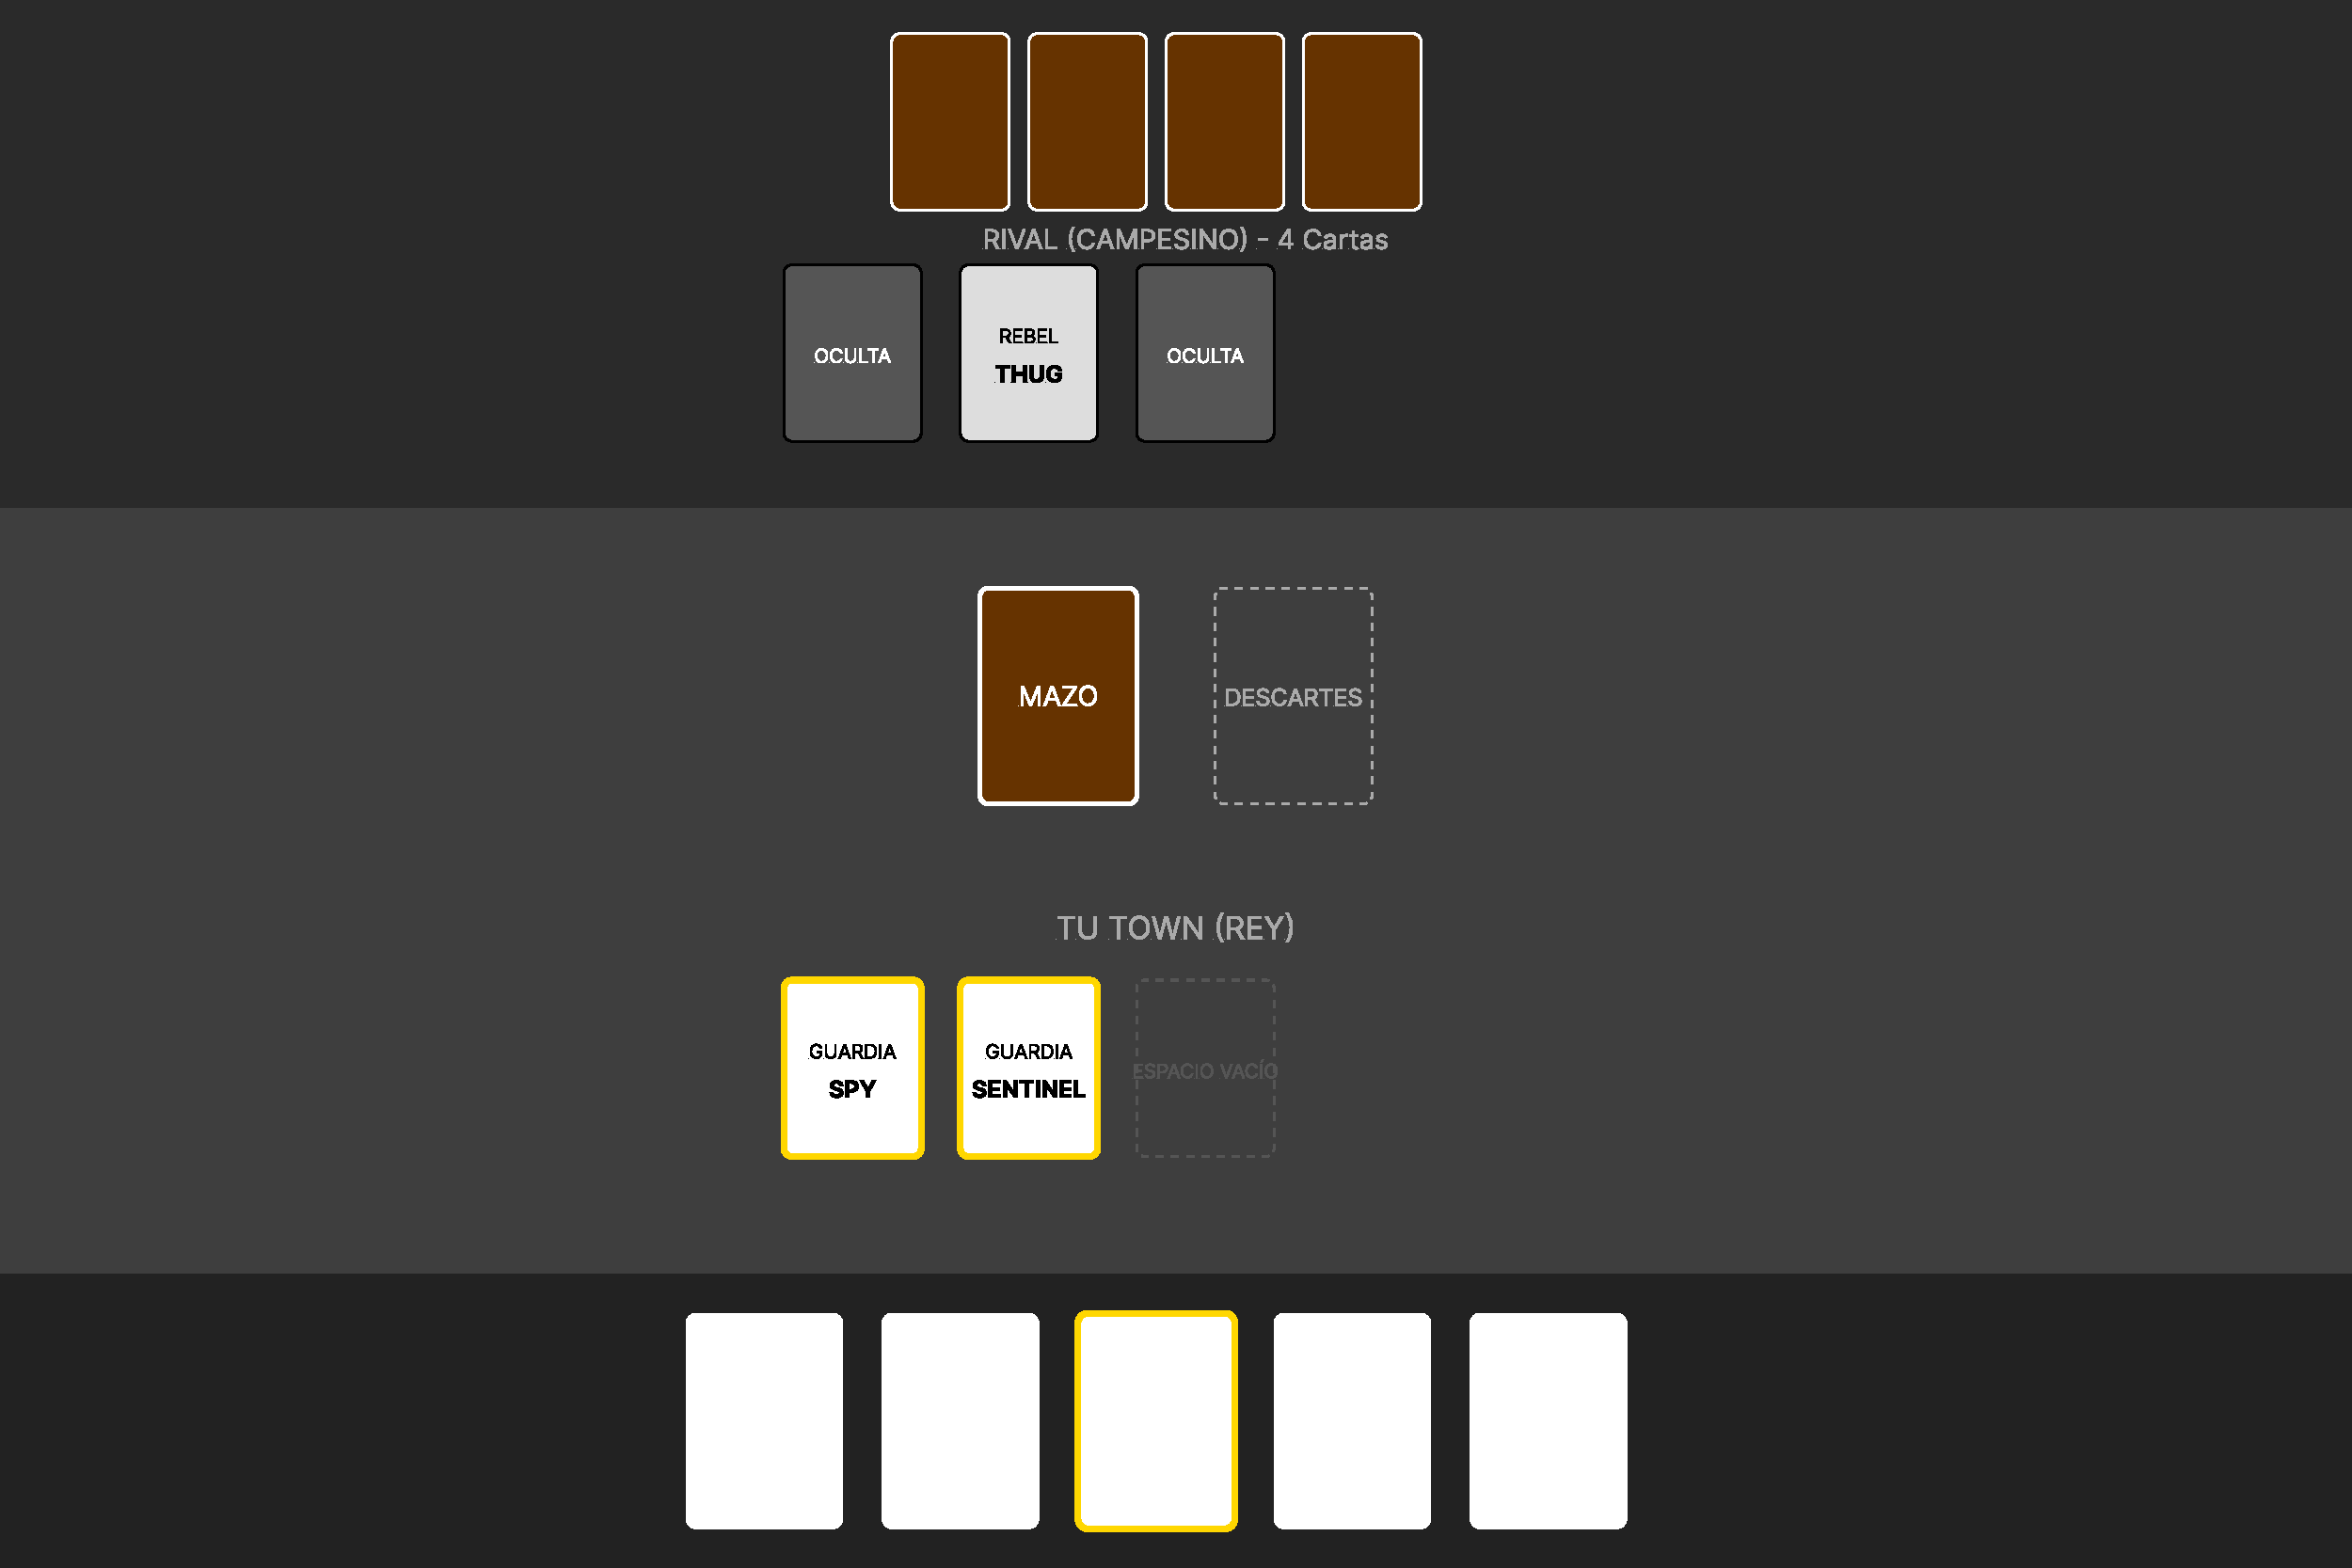
\includegraphics[width=0.9\textwidth]{figures/game_board_ui.pdf}
\caption{Captura de los mock-ups de la interfaz principal: Tablero de juego asimétrico y salas de espera (Lobbies).}
\label{fig:ui_gameboard}
\end{center}
\end{figure}

\textbf{3. Detalles de Implementación} \\
La integración de múltiples motores de bases de datos exigió un desarrollo cauteloso en el archivo \texttt{docker-compose.yml}. Se implementaron volúmenes persistentes (\textit{Volumes}) tanto para \textit{MariaDB} (\texttt{/var/lib/mysql}) como para \textit{Redis} (\texttt{/data}), asegurando que la reinicialización de los contenedores no provocara la pérdida de información crítica. Adicionalmente, se ejecutaron comprobaciones de estado (\textit{healthchecks}) con comandos nativos como \textit{mysqladmin ping} y \textit{redis-cli ping}, garantizando que los servicios de \textit{backend} dependientes (\textit{depends\_on}) no intenten establecer conexiones hasta que los motores estén operativos.

\textbf{4. Seguimiento, Control y Replanificación} \\
Durante el control de la integración del almacenamiento en memoria surgieron bloqueos temporales en la comunicación de los servicios locales. La desviación se resolvió en caliente corrigiendo el mapeo de puertos y exponiendo el 6379 hacia el \textit{localhost} en el \texttt{docker-compose.yml}. Tras esta corrección, las tareas se completaron satisfactoriamente y se integraron en la rama principal, dejando la plataforma preparada para iniciar la estructuración del ORM en la iteración siguiente.

\section{Autenticación y Modelado de Datos}

\textbf{Flujo de Interacción y Arquitectura} \\
El flujo de autenticación implementa el patrón de diseño \textit{Context API} en el \textit{frontend} para inyectar globalmente el estado de sesión del usuario. A nivel de \textit{backend}, se utiliza \textit{Prisma ORM} como intermediario transaccional con la base de datos relacional. Las peticiones a rutas protegidas se validan mediante \textit{middlewares} que decodifican \textit{JSON Web Tokens (JWT)}, logrando una arquitectura de seguridad robusta y desacoplada.

\textbf{Estructura de Directorios} \\
\begin{verbatim}
packages/
|-- client/src/
|   +-- context/
|       +-- AuthContext.ts
+-- server/
    |-- prisma/
    |   +-- schema.prisma
    +-- src/controllers/
        +-- UserController.js
\end{verbatim}

\textbf{Snippets Estratégicos de Código} \\
\begin{lstlisting}[language=Java]
// packages/client/src/context/AuthContext.ts
interface AuthContextType {
  user: User | null;
  isLogin: boolean;
  login: (userData: User) => void;
  // ... logica interna omitida para resumir el contenido
  socket: Socket | null;
}
export const AuthContext = createContext<AuthContextType | undefined>(undefined);
\end{lstlisting}

\begin{lstlisting}[language=Java]
// packages/server/prisma/schema.prisma
model User {
  idUser   Int      @id @default(autoincrement())
  name     String   @unique
  email    String   @unique
  password String
  // ... resto de campos relacionales omitidos
}
\end{lstlisting}

\subsection{Iteración 3: Modelado Estructural y Flujo de Negocio}

\textbf{1. Definición de Características} \\
El objetivo principal asignado para esta iteración se centró en la conceptualización teórica del dominio de datos, así como en el modelado formal del flujo que gobernaría la asimetría de las partidas.

\textbf{2. Diseño de la Solución} \\
El diseño de esta etapa se articuló en torno a la arquitectura de la información. Se elaboró el modelo Entidad-Relación y el diagrama UML correspondiente a la base de datos relacional. De forma paralela, el equipo diseñó los estados de la partida, los turnos intercalados y las mecánicas asimétricas plasmándolas en diagramas de flujo operativos.

\textbf{3. Detalles de Implementación} \\
El diseño estructural requirió abstraer la asimetría del juego a un modelo de datos cohesivo. El esquema relacional implementó entidades independientes para \texttt{User}, \texttt{Friendship}, \texttt{Lobby} y \texttt{Game}. La complejidad se centró en la entidad \texttt{Card}, la cual fue codificada para contener tanto los atributos del bando del Rey (\texttt{nameKing}, \texttt{typeKing}) como los del Campesino (\texttt{namePeasant}, \texttt{typePeasant}) en un mismo registro. Esto facilitó enormemente la futura gestión del mazo único compartido. Las relaciones múltiples reflexivas en la entidad \texttt{User} (como \texttt{gamesAsPlayer1} o \texttt{friendshipsSent}) se implementaron para permitir consultas eficientes de historiales y marcadores.

\textbf{4. Seguimiento, Control y Replanificación} \\
El seguimiento de este \textit{sprint} arrojó resultados óptimos. Los objetivos de modelado de datos y flujos lógicos se alcanzaron con éxito, sin registrarse desviaciones temporales ni bloqueos técnicos que obligaran a replanificar. El diseño quedó certificado y listo para ser trasladado al ORM en la siguiente iteración.

\subsection{Iteración 4: Implementación del Modelo Estructural para los usuarios}

\textbf{1. Definición de Características} \\
El objetivo principal para esta iteración se basó en la implementación técnica del modelo de datos diseñado previamente en la base de datos relacional, haciendo uso del modelo Entidad-Relación y el diagrama UML correspondiente.

\textbf{2. Diseño de la Solución} \\
En cumplimiento con el requisito de arquitectura (\textbf{RNF-ARQ}), el diseño de la solución dictaminó que este modelo conceptual se trasladara al entorno de desarrollo utilizando \textit{Prisma ORM}. Se diseñó una estrategia basada en migraciones secuenciales sobre el despliegue aislado de \textit{MariaDB}, garantizando que el esquema de la base de datos estuviera en sincronía con el contenedor de Docker.

\textbf{3. Detalles de Implementación} \\
La transición del modelo a la infraestructura real se codificó definiendo el esquema en \texttt{schema.prisma}. Esta implementación generó automáticamente un cliente tipado para \textit{Node.js}, proporcionando autocompletado y seguridad de tipos en la capa de controladores. La ejecución de las migraciones (\texttt{prisma migrate}) actuó como un sistema de control de versiones sobre \textit{MariaDB}, garantizando que cualquier cambio en la estructura de tablas o índices (como \texttt{@@unique([idSender, idReceiver])} en las amistades) se aplicase de forma atómica.

\textbf{4. Seguimiento, Control y Replanificación} \\
Durante el control de calidad de la iteración no se reportaron fallos en las transacciones de las migraciones. El modelo de datos se materializó en los contenedores locales sin desviaciones, cerrando la iteración en el tiempo estipulado y permitiendo continuar con la capa de seguridad.

\subsection{Iteración 5: Gestión de Identidad, Seguridad y Perfiles}

\textbf{1. Definición de Características} \\
El objetivo primordial de este ciclo consistió en implementar de forma integral la capa de gestión de usuarios del ecosistema. Esto abarcó tanto la seguridad del acceso (registro y autenticación de credenciales) como la administración de la identidad digital del jugador, proporcionando una zona privada para la edición de datos personales y la visualización de estadísticas de juego.

\textbf{2. Diseño de la Solución} \\
El diseño de la solución abordó la construcción de las vistas operativas de \textit{Login}, \textit{Register} y el panel de \textit{Profile}. Dando cumplimiento al requisito de seguridad (\textbf{RNF-SEG}), el diseño de la lógica del servidor se basó en la emisión y validación de \textit{JSON Web Tokens} (JWT), asegurando el encriptado unidireccional de contraseñas. Para el cliente, se diseñaron formularios reactivos integrados con un contexto global de autenticación para gobernar las rutas privadas.

\textbf{3. Detalles de Implementación} \\
El núcleo de la seguridad se implementó codificando la ofuscación de contraseñas con \textit{bcrypt} durante el registro. En la autenticación exitosa, el \textit{backend} firma un JWT empaquetando el identificador del usuario. El \textit{frontend} inyecta este \textit{token} como cabecera en cada petición HTTP protegida. Un \textit{middleware} programado en \textit{Node.js} intercepta estas peticiones, verificando la validez criptográfica de la firma antes de permitir el acceso a controladores restringidos mediante \textit{Prisma ORM}.

\textbf{4. Seguimiento, Control y Replanificación} \\
El seguimiento de la integración detectó desviaciones severas en el cliente y el servidor. En el \textit{frontend}, surgieron dificultades con la persistencia del estado de sesión; se replanificó implementando un \textit{AuthContext} en \textit{React}. En el \textit{backend}, el diseño inicial de los controladores mezclaba validaciones con persistencia. Se aplicó una refactorización correctiva orientada a la separación de responsabilidades. Tras estas acciones de control, la iteración concluyó satisfactoriamente unificando los flujos de acceso.

\section{Interacciones Sociales y Comunicación Bidireccional}

\textbf{Flujo de Interacción y Arquitectura} \\
Para resolver la latencia en la interacción social (sistema de amigos y futuras mecánicas de partida), se sustituye el modelo tradicional de \textit{HTTP Polling} por una conexión persistente bidireccional basada en el protocolo \textit{WebSockets} utilizando \textit{Socket.io}. La arquitectura se modela mediante un \textit{Socket Manager} en el servidor, implementado bajo un patrón \textit{Singleton}, que gestiona la emisión de eventos (\textit{Broadcast}) a salas específicas y propaga notificaciones en tiempo real a los clientes conectados.

\textbf{Estructura de Directorios} \\
\begin{verbatim}
packages/server/src/
|-- controllers/
|   +-- FriendshipController.js
+-- sockets/
    +-- LobbySocket.js
\end{verbatim}

\textbf{Snippets Estratégicos de Código} \\
\begin{lstlisting}[language=Java]
// packages/server/src/sockets/LobbySocket.js
const registerLobbyHandlers = (io, socket) => {
  // ... configuracion interna omitida para resumir el contenido
  socket.on("createLobby", async (lobbyName, isPrivate) => {
      // ... logica de emision de eventos omitida
  });
}
\end{lstlisting}

\subsection{Iteración 6: Interacciones Sociales y Comunicación en Tiempo Real}

\textbf{1. Definición de Características} \\
El objetivo establecido para este ciclo fue implementar el componente social del ecosistema, diseñando un sistema de amistades entre usuarios e introduciendo la base técnica para la comunicación bidireccional necesaria en la futura partida.

\textbf{2. Diseño de la Solución} \\
El diseño se dividió en dos frentes. Por un lado, se planificaron los \textit{endpoints} y el modelo de entidad relacional para enviar, aceptar y rechazar amistades, junto con su vista (\textit{Dashboard}). Por otro lado, en cumplimiento del requisito de rendimiento (\textbf{RNF-REN}), se diseñó la sustitución del protocolo HTTP tradicional por \textit{WebSockets} (\textit{Socket.io}) en el servidor. La justificación arquitectónica de esta decisión se detalla en la Tabla \ref{tab:ws_analisis}.

\begin{table}[H]
\centering
\begin{coolTable}{p{4cm}p{\textwidth-4.5cm}}{2}
{Análisis de valor: Comunicación por WebSockets}
\textbf{Propuesta}&Sustitución del paradigma HTTP tradicional (REST) por un canal persistente bidireccional basado en Socket.io.\\
\midrule
\textbf{Valor}&Garantiza latencia casi nula para la sincronización de las mecánicas de partida y notificaciones de amistad.\\
\textbf{Coste}&Aumenta la complejidad de la infraestructura al requerir un \textit{Socket Manager} y mayor consumo de memoria por conexiones abiertas.\\
\textbf{Opciones}&\textit{HTTP Long Polling} o \textit{Server-Sent Events (SSE)}, descartadas por sobrecarga de red y limitación unidireccional respectivamente.\\
\textbf{Riesgos}&Riesgo crítico de fugas de memoria (\textit{memory leaks}) ante desconexiones no gestionadas de los clientes.\\
\textbf{Deuda técnica}&Obliga a implementar lógicas manuales de reconexión y ciclos de limpieza (\textit{cleanup}) en el frontend (React).\\
\end{coolTable}
\caption{Análisis de valor aportado sobre la arquitectura de comunicación mediante WebSockets. \label{tab:ws_analisis}}
\end{table}

\textbf{3. Detalles de Implementación} \\
El principal desafío de implementación consistió en mantener una única fuente de verdad sincronizada. El algoritmo desarrollado operó estableciendo un mapa en memoria en el servidor que vincula el \texttt{userId} con su \texttt{socket.id}. Tras completarse una transacción en \textit{MariaDB} (ej. aceptar una solicitud), el controlador invoca al gestor de \textit{Sockets}. Éste emite un evento tipado (\textit{Broadcast} dirigido) enviando el nuevo estado del \textit{Dashboard}, forzando a la vista \textit{React} a re-renderizarse de forma reactiva sin necesidad de sondeo.

\textbf{4. Seguimiento, Control y Replanificación} \\
Durante el control de calidad de la comunicación, se detectaron dificultades persistentes para establecer una conexión estable (fugas de memoria por múltiples instancias por usuario). La desviación se mitigó replanificando la lógica del cliente e implementando retornos de limpieza (\textit{cleanup}) en los \textit{hooks} de \textit{React} para forzar la desconexión explícita. El ciclo concluyó exitosamente, dejando el motor de comunicación listo para iniciar el flujo principal de la partida.

\section{Arquitectura del Motor de Juego Asimétrico}

\textbf{Flujo de Interacción y Arquitectura} \\
El núcleo funcional del proyecto delega el estado asimétrico de las partidas a un servicio especializado (\textit{Game Service}) que interactúa con la base de datos en memoria \textit{Redis} para minimizar la latencia. El intercambio de información entre servidor y cliente se rige por Objetos de Transferencia de Datos (\textit{DTO}), filtrando atributos confidenciales antes de emitir actualizaciones por \textit{WebSockets}. Las mecánicas asíncronas, como \textit{Pending Actions}, pausan y retoman el hilo de ejecución mediante identificadores únicos.

\textbf{Estructura de Directorios} \\
\begin{verbatim}
packages/
|-- client/src/pages/game/
|   +-- components/
|       +-- GameService.tsx
+-- server/src/
    |-- services/
    |   +-- GameService.js
    +-- controllers/
        +-- GameController.js
\end{verbatim}

\textbf{Snippets Estratégicos de Código} \\
\begin{lstlisting}[language=Java]
// packages/server/src/services/GameService.js
const playActionCard = async (gameId, targetData, playedCard, userRol, gameState) => {
  // ... logica interna de validacion y estado en Redis omitida
}
  
const resolvePendingAction = async (gameId, userId, targetData) => {
  // ... logica de resolucion transaccional omitida
}
\end{lstlisting}

\subsection{Iteración 7: Documentación, Planificación y QA}

\textbf{1. Definición de Características} \\
El objetivo inicial de la iteración consistía en comenzar el desarrollo técnico del motor de juego y el chat en partida. Sin embargo, ante el rápido crecimiento del proyecto, el equipo decidió estratégicamente pivotar los esfuerzos hacia una auditoría profunda del código existente, evaluando las funcionalidades implementadas hasta la fecha para identificar y catalogar la deuda técnica acumulada.

\textbf{2. Diseño de la Solución} \\
Al paralizar el desarrollo de nuevas características, el diseño se centró en elaborar un plan de auditoría. Dando cumplimiento al requisito de mantenibilidad (\textbf{RNF-MAN}), se diseñó un protocolo de revisión de los flujos de datos entre cliente y servidor, con el fin de detectar problemas de escalabilidad visual y riesgos de sobreexposición de datos sensibles en red que podrían comprometer la arquitectura asimétrica futura.

\textbf{3. Detalles de Implementación} \\
Durante este periodo, la ejecución técnica se limitó a tareas de inspección de código estático y análisis de tráfico de red. Se identificaron vulnerabilidades estructurales en la serialización de datos enviados por \textit{WebSockets} y un alto nivel de acoplamiento en los componentes de \textit{React}, documentando exhaustivamente cada hallazgo en el sistema de control de versiones (\textit{Issues}).

\textbf{4. Seguimiento, Control y Replanificación} \\
El control de este \textit{sprint} representó un punto de inflexión crítico. La auditoría demostró que era inasumible continuar el desarrollo sin sanear el núcleo del sistema. Como medida de replanificación, el equipo modificó la pila de producto (\textit{Product Backlog}), arrastrando el desarrollo del chat y priorizando una refactorización masiva para el siguiente ciclo. Se asumió el riesgo consciente de que ciertas características menores quedarían fuera del alcance del proyecto a cambio de garantizar la integridad de la arquitectura central.

\subsection{Iteración 8: Refactorización y Estado Inicial de Partida}

\textbf{1. Definición de Características} \\
El objetivo de este \textit{sprint} fue ejecutar la reestructuración profunda dictaminada en la auditoría previa para mejorar la legibilidad del código. Adicionalmente, se fijó el hito de preparar la base de datos para la configuración del estado inicial de la partida (cartas y mazos).

\textbf{2. Diseño de la Solución} \\
Para cumplir el requisito de mantenibilidad (\textbf{RNF-MAN}), el diseño de la refactorización dictó unificar la nomenclatura y extraer componentes reutilizables en \textit{React}. A nivel de arquitectura (\textbf{RNF-ARQ}), se diseñó el uso del patrón \textit{Data Transfer Object} (DTO) para aislar la \textit{lógica de negocio} de los datos emitidos por red, asegurando la naturaleza "ciega" del juego asimétrico. Además, se planificaron los \textit{seeders} de la base de datos.

\textbf{3. Detalles de Implementación} \\
La vulnerabilidad estructural descubierta se mitigó codificando funciones adaptadoras (\textit{mappers}) puras. Estas rutinas reciben el estado absoluto del juego desde \textit{Redis} y construyen un nuevo objeto purgado para el \textit{socket} receptor. De este modo, propiedades sensibles como la mano del rival se procesan y se envían únicamente como conteos de longitud (números enteros), garantizando que el cliente no pueda inspeccionar el tráfico para obtener ventajas ilícitas.

\textbf{4. Seguimiento, Control y Replanificación} \\
Durante la validación de la refactorización, el seguimiento reveló brechas en el filtrado de datos (ej. \textit{Rival town dto}), que seguían exponiendo información privada. El control de calidad forzó a replanificar la serialización JSON, introduciendo validadores estrictos en los \textit{mappers}. Tras superar este reto, la base de código quedó notablemente robusta y lista para iniciar el sistema funcional de cartas.

\subsection{Iteración 9: Desarrollo del Motor de Juego y Cartas de Acción}

\textbf{1. Definición de Características} \\
El objetivo establecido consistió en dotar de vida al motor de \textit{King and Peasant}, centrándose en la implementación funcional de las cartas de acción y el complejo sistema de acciones pendientes (\textit{Pending Actions}) para manejar la interactividad asimétrica de la partida.

\textbf{2. Diseño de la Solución} \\
El diseño de la solución abordó la creación de los servicios (\textit{Game Service}) y controladores encargados de procesar el uso de cartas, validando la capacidad asimétrica del tablero (\textbf{RN-02}) y automatizando el cierre de turno (\textbf{RN-04}). En el cliente, se diseñaron las interfaces dinámicas para explorar la pila de descartes y el diccionario visual de acciones.

\textbf{3. Detalles de Implementación} \\
El problema computacional residía en congelar el estado del motor de forma segura delegando el contexto a \textit{Redis}. El sistema de cola de acciones (\textit{Pending Actions}) se implementó generando un objeto \texttt{pendingAction} que bloquea algorítmicamente el turno global. Cuando el cliente envía la resolución, un despachador dinámico invoca la función específica requerida, aplica las mutaciones, purga la acción y reactiva el turno, tal y como se formaliza en la Tabla \ref{tab:pending_actions}.

\begin{table}[htbp]
\centering
\begin{asigResponsabilidad}{game-001}{Resolución Pending Actions}
{[Object] resolvePendingAction (gameId:String, userId:Int, targetData:Object)}
\pasoPseudo{Recuperar el estado actual (\texttt{gameState}) almacenado en Redis mediante el \texttt{gameId}.}
\pasoPseudo{Validar que el \texttt{userId} de la petición coincide con el jugador que tiene el foco activo en el objeto \texttt{pendingAction}.}
\pasoPseudo{Invocar al despachador de cartas para aplicar el efecto mecánico sobre el \texttt{targetData}.}
\pasoPseudo{Si la resolución es exitosa, aplicar las mutaciones y purgar el objeto \texttt{pendingAction} del estado general.}
\pasoPseudo{Transicionar el foco y guardar el nuevo estado atómico en Redis.}
\end{asigResponsabilidad}
\caption{Descripción algorítmica de la resolución de acciones asíncronas en el servidor. \label{tab:pending_actions}}
\end{table}

\textbf{4. Seguimiento, Control y Replanificación} \\
El control de la implementación reportó complicaciones severas al sincronizar las mecánicas asíncronas del servidor con la vista. Al aplicar reglas estrictas (\textbf{RN-03}), se originaron bloqueos en la selección de cartas. La desviación obligó a replanificar el control de flujo en \textit{React}, aislando la resolución de las promesas del ciclo de vida de los modales. Solventado esto, el hito crítico se alcanzó, permitiendo la interactividad en mesa.

\subsection{Iteración 10: Condiciones de Victoria y Resolución de Partida}

\textbf{1. Definición de Características} \\
El objetivo fue definir la finalización algorítmica de las partidas, estableciendo las condiciones de victoria asimétricas de cada facción (Guardias vs. Asesino/Revueltas) y puliendo mecánicas clave de final de juego.

\textbf{2. Diseño de la Solución} \\
Para garantizar la atomicidad de victoria (\textbf{RN-05}), el diseño de la lógica de negocio exigió que el motor comprobara de forma asíncrona la victoria tras cada movimiento. Se ideó una orquestación transaccional para asegurar que, al detectar un ganador, \textit{MariaDB} reflejara el cambio de estado, la caché en memoria se bloqueara y el cliente renderizara modales dinámicos de cierre.

\textbf{3. Detalles de Implementación} \\
La complejidad se abordó programando un interceptor central de validación. Tras cualquier mutación en \textit{Redis}, el algoritmo evalúa en paralelo las condiciones absolutas del Campesino frente a las del Rey. Si una aserción retorna un estado ganador válido, el motor consolida el estado en \textit{MariaDB} dentro de una misma transacción de \textit{Prisma}, y envía un código de interrupción por \textit{WebSockets} que destruye el hilo de memoria para evitar condiciones de carrera.

\textbf{4. Seguimiento, Control y Replanificación} \\
Durante las pruebas de transición final, el equipo de control detectó errores de concurrencia que desencadenaban un Error 500 en el servidor al intentar actualizar el estado y destruir el hilo simultáneamente. La corrección requirió replanificar el \texttt{GameController}, encapsulando las sentencias en un bloque transaccional \textit{try/catch} con \textit{await}. Tras la corrección, el motor logró determinar a un ganador de forma robusta.

\section{Aseguramiento de Calidad y Pulido Final}

\textbf{Flujo de Interacción y Arquitectura} \\
La estrategia de validación final adopta un enfoque orientado al aseguramiento de la calidad mediante pruebas de integración automáticas. A nivel de infraestructura, se utiliza el motor \textit{Jest} para instanciar el \textit{Game Service} y los servicios de usuarios junto con bases de datos aisladas en memoria. Esto permite simular con precisión el flujo asimétrico de la partida, certificando la invariabilidad algorítmica de las condiciones de victoria y mitigando la aparición de regresiones indeseadas tras refactorizaciones de última hora.

\textbf{Estructura de Directorios} \\
\begin{verbatim}
packages/
+-- server/
    +-- tests/
        |-- gameService.test.mjs
        |-- userRoutes.test.mjs
        +-- userService.test.mjs
\end{verbatim}

\textbf{Snippets Estratégicos de Código} \\
\begin{lstlisting}[language=Java]
// packages/server/tests/gameService.test.mjs
describe('gameService', () => {
  test('startGame inicializa la partida correctamente con las reglas de King and Peasant', async () => {
     // ... logica interna de aserciones y simulacion omitida
  });
});
\end{lstlisting}

\subsection{Iteración 11: Interfaces Asíncronas y Modales de Cartas de Acción}

\textbf{1. Definición de Características} \\
El objetivo fundamental consistió en desarrollar la capa visual e interactiva del núcleo del juego, implementando el \textit{frontend} de las Cartas de Acción y el complejo sistema de Acciones Pendientes (\textit{Pending Actions}) para permitir a los jugadores reaccionar a eventos asimétricos.

\textbf{2. Diseño de la Solución} \\
Para cumplir el requisito de rendimiento (\textbf{RNF-REN}), el diseño planteó traducir la lógica del servidor a una experiencia reactiva. Se proyectó un diccionario visual unificado (\texttt{pendingActionsUI.tsx}) capaz de instanciar modales específicos (como el ataque \textit{Strike} del Rey) congelando la interfaz general sin perder el contexto visual del tablero.

\textbf{3. Detalles de Implementación} \\
El diccionario dinámico se implementó mapeando las claves de acción del servidor con sus respectivos componentes en \textit{React}. Cuando \textit{Socket.io} notifica un estado con \texttt{pendingAction}, el cliente evalúa si el foco recae en el jugador local. En caso afirmativo, se invoca el componente del diccionario forzando la decisión del usuario y bloqueando algorítmicamente el resto de interacciones (\textit{force play}) hasta que el controlador del servidor resuelva la promesa asíncrona.

\textbf{4. Seguimiento, Control y Replanificación} \\
Durante el acoplamiento del diccionario, el control de la interfaz detectó desajustes visuales (\textit{frontend bugs}) al intentar interactuar con el mazo general mientras un modal estaba activo. Este defecto forzó una replanificación en la jerarquía de dependencias de \textit{React}, reescribiendo los \textit{hooks} para forzar el paso de turno únicamente cuando se confirmaba el retorno HTTP/WS 200 desde el servidor, estabilizando así el flujo.

\subsection{Iteración 12: Consolidación Funcional del Motor de Juego y Lógica de Cartas}

\textbf{1. Definición de Características} \\
El propósito consistió en consolidar el abanico completo de funcionalidades mecánicas de las cartas de ambos bandos, asegurando que las acciones asimétricas complejas (como tácticas de guardias o emboscadas) se resolvieran de forma íntegra.

\textbf{2. Diseño de la Solución} \\
Dando cumplimiento al requisito de funcionalidad (\textbf{RNF-FUN}), el diseño algorítmico orquestó rutinas para alterar el estado de las entidades, calcular daños, escudos y penalizaciones de forma atómica. En el \textit{frontend}, el diseño contempló la incorporación de modales dinámicos para visualizar mazos durante la partida.

\textbf{3. Detalles de Implementación} \\
La programación de acciones múltiples (ej. una carta que permite mirar la mano rival y descartar una carta) se implementó bifurcando el \textit{GameService}. El servidor valida la orden y crea el \texttt{pendingAction}, inyectando al cliente los datos temporales. Una vez tomada la decisión, la resolución final unifica las propiedades alteradas y reanuda el turno general purgando la caché diferida de \textit{Redis}, garantizando una ejecución inmutable.

\textbf{4. Seguimiento, Control y Replanificación} \\
El control de calidad evidenció fricciones temporales al enlazar el diccionario visual con resoluciones múltiples encadenadas. Las respuestas de validación fallaban. Como medida correctiva, se replanificó la arquitectura de respuestas del \textit{GameService} para homogeneizar los formatos de transferencia (DTO) en cada paso de validación intermedia, dejando el sistema de cartas prácticamente completado.

\subsection{Iteración 13: Interfaces de Infiltración y Estabilización del Bucle de Partida}

\textbf{1. Definición de Características} \\
El objetivo fue completar la capa de presentación de la mecánica especial de Infiltración y garantizar la robustez algorítmica del bucle de partida (transiciones entre Eras y validaciones deterministas).

\textbf{2. Diseño de la Solución} \\
Para asegurar la fiabilidad (\textbf{RNF-FIA}), el diseño requirió crear un componente reactivo (\texttt{InfiltrateModal.tsx}) acoplado al diccionario de acciones, dotando al jugador de una vista controlada para examinar la mano rival. Paralelamente, se diseñó la estabilización de los scripts de entorno local (\texttt{npm run start:local}) y del bloque de aserciones de victoria (\textit{Win Condition}) en el servidor.

\textbf{3. Detalles de Implementación} \\
El componente \textit{React} fue programado para capturar el DTO efímero y congelar el entorno de la partida. Su estado visual se coordinó estrictamente con la respuesta asíncrona del servidor, asegurando que los modales se desmontaran limpiamente y reanudaran el cauce natural de turnos tras la alteración exitosa en la base de datos de memoria.

\textbf{4. Seguimiento, Control y Replanificación} \\
Las pruebas del bucle final de juego levantaron una alerta crítica: la invocación a \texttt{setupNewEra} corrompía la asignación de cartas en memoria al cambiar de fase. La desviación exigió replanificar los ciclos del \textit{GameService}, reescribiendo desde cero las funciones de reasignación y limpieza de manos para asegurar que la nueva Era comenzara de forma determinista.

\subsection{Iteración 14: Pulido de Reglas, Corrección de Errores y Refactorización Estructural}

\textbf{1. Definición de Características} \\
El propósito central consistió en el pulido exhaustivo de las reglas del juego (Guardias, Revueltas, Asesino) y el arreglo de errores arrastrados. Además, se fijó el objetivo de optimizar la mantenibilidad del código (\textbf{RNF-MAN}) del \textit{frontend}.

\textbf{2. Diseño de la Solución} \\
El diseño para refactorizar la excesiva complejidad del componente principal (\texttt{Game.tsx}) se fundamentó en tres pilares: extraer la lógica transaccional a \textit{Custom Hooks}, descomponer el árbol JSX en componentes atómicos (\texttt{PlayerArea.tsx}, \texttt{RivalArea.tsx}), y encapsular todas las interfaces de interrupción (\textit{Modals}) para mitigar re-renderizados.

\textbf{3. Detalles de Implementación} \\
A nivel de reglas, se programaron las correcciones matemáticas en los cálculos de letalidad. En la capa de \textit{frontend}, la refactorización se materializó separando el estado global de suscripciones a \textit{WebSockets} hacia \texttt{useGameActions.ts} y \texttt{useGameData.ts}. Adicionalmente, se codificó un nuevo sistema de notificaciones (\texttt{ErrorToast.tsx}) para interceptar y renderizar los errores enviados por el servidor.

\textbf{4. Seguimiento, Control y Replanificación} \\
Durante las pruebas de estrés de este ciclo, el control de errores cazó un fallo 500 no controlado en el cierre de sesiones. Este defecto crítico se solucionó encapsulando el cierre de la partida en una gestión robusta de excepciones. Esta acción correctiva dejó una base limpia y altamente estable.

\subsection{Iteración 15: Sistema de Notificaciones Globales y Alertas de Partida}

\textbf{1. Definición de Características} \\
El objetivo técnico fue interceptar eventos asíncronos críticos transversales (como la finalización oficial de una partida o el abandono de salas de espera) y comunicarlos de forma inmediata mediante modales reactivos, mejorando el \textit{feedback} global.

\textbf{2. Diseño de la Solución} \\
Dando cumplimiento al requisito de usabilidad, el diseño propuso la creación del componente \texttt{AnnouncementModal.tsx}. La arquitectura planificó inyectarlo en la capa superior de la aplicación para interceptar los estados tanto en \texttt{Game.tsx} como en \texttt{LobbyRoom.tsx}, manteniéndolo oculto por defecto.

\textbf{3. Detalles de Implementación} \\
La integración se programó ampliando el estado global en los \textit{hooks} personalizados para escuchar de forma activa las interrupciones de \textit{Socket.io}. Al emitirse una notificación de victoria o abandono, el motor reactivo de estado dispara el modal, bloqueando la interfaz subyacente para forzar la navegación del usuario hacia una zona segura (como el menú principal) e invalidando las interacciones residuales.

\textbf{4. Seguimiento, Control y Replanificación} \\
El seguimiento de la implementación reportó conflictos de renderizado: el modal retenía información obsoleta tras salidas abruptas de los \textit{Lobbies}. La solución requirió replanificar el ciclo de vida de desmontaje en \textit{React}, añadiendo lógicas estrictas para purgar las suscripciones a \textit{WebSockets} antes de destruir la vista. Tras esto, las notificaciones funcionaron de forma impecable.

\subsection{Iteración 16: Automatización de Pruebas y Validación Integral del Sistema}

\textbf{1. Definición de Características} \\
El objetivo de este \textit{sprint} se centró en asegurar la calidad del software mediante la automatización de pruebas, blindando la \textit{lógica de negocio} del motor asimétrico y las interfaces, garantizando así la fiabilidad (\textbf{RNF-FIA}) del producto.

\textbf{2. Diseño de la Solución} \\
Se diseñó una \textit{suite} de pruebas utilizando el motor \textit{Jest}. La arquitectura de validación simuló servicios de usuarios y el \textit{Game Service} operando contra bases de datos aisladas en memoria. En \textit{frontend}, el diseño abarcó pruebas de componentes mediante DOM virtual para verificar los flujos de inicio de sesión y gestión de perfil.

\textbf{3. Detalles de Implementación} \\
Las pruebas automatizadas lograron exponer fragilidades en lógicas de cascada (como \textit{Revolt}). La refactorización exigió aislar las mutaciones de poder en buffers temporales. Se codificó una resolución en cascada estricta, asegurando que los eventos masivos no sobreescribieran referencias de memoria. Esta aproximación garantizó que, si el sistema asíncrono detectaba un fallo, la operación atómica abortara preservando la partida intacta.

\textbf{4. Seguimiento, Control y Replanificación} \\
Durante el monitoreo de la \textit{suite}, el sistema reportó discrepancias graves en \textit{Redis}: mecánicas letales (\textit{Strike}) no aplicaban el daño correctamente. El equipo pausó la creación de nuevos \textit{tests} y replanificó el esfuerzo para reescribir parte de la lógica en los \textit{pendingActions} defectuosos. Tras iterar sobre el código, la tasa de éxito de las pruebas alcanzó el 100\%, validando la estabilidad definitiva del software.

\subsection{Iteración 17: Redacción Técnica y Consolidación Documental}

\textbf{1. Definición de Características} \\
El objetivo primordial de este ciclo final consistió en intensificar la producción de la memoria técnica del proyecto, liberando ancho de banda y presión administrativa para afrontar la entrega definitiva.

\textbf{2. Diseño de la Solución} \\
La solución metodológica planteó detener el desarrollo de nuevas características y establecer un flujo de redacción concurrente. El diseño documental exigió justificar las decisiones arquitectónicas previas y estructurar todos los artefactos visuales (diagramas UML, tablas de análisis) generados a lo largo de los 16 \textit{sprints} anteriores.

\textbf{3. Detalles de Implementación} \\
La ejecución se centró en el trabajo sobre el proyecto \textit{LaTeX}. Se unificó el estilo narrativo del equipo y se resolvieron errores tipográficos y de compilación (\textit{Overfull hboxes}). La redacción se abordó con revisiones cruzadas constantes frente al repositorio de código fuente para garantizar que la memoria fuera un reflejo técnico exacto de la ingeniería de \textit{King and Peasant}.

\textbf{4. Seguimiento, Control y Replanificación} \\
El control de la iteración no reportó bloqueos de software, pero evidenció la carga cognitiva de transicionar del código a la redacción académica. La gestión del tiempo se ajustó mediante sesiones cortas de validación, logrando completar la estructura de la memoria sin desviaciones temporales. El ciclo cerró el cronograma de iteraciones con un éxito rotundo.
\chapter{Pruebas y Validación del Sistema}

En este capítulo se describe la estrategia de verificación adoptada para asegurar la calidad y el correcto funcionamiento de la plataforma \textit{King and Peasants}. Se detalla el diseño de las pruebas siguiendo una arquitectura de pirámide, la validación de los componentes de interfaz, la integridad de la API y el motor de lógica asimétrica, así como el flujo de integración continua que garantiza la estabilidad en cada despliegue.

\section{Estrategia de Pruebas y Entorno}

Se ha diseñado una estrategia de pruebas integral que abarca desde la lógica de negocio más granular hasta el comportamiento de la interfaz de usuario. El stack tecnológico de pruebas se divide según la naturaleza de cada paquete:

\begin{itemize}
    \item \textbf{Cliente (\textit{frontend}):} Se utiliza \textbf{Vitest} como motor de ejecución de pruebas por su integración nativa con Vite, junto con \textbf{React Testing Library (RTL)} para la validación de componentes basada en el comportamiento del usuario.
    \item \textbf{Servidor (\textit{backend}):} Se emplea \textbf{Jest} para la ejecución de pruebas unitarias y de integración, complementado con \textbf{Supertest} para la realización de peticiones HTTP sintéticas contra los \textit{endpoints} de la API.
\end{itemize}

La pirámide de pruebas implementada asegura que la base del sistema esté cubierta por pruebas unitarias rápidas y ligeras, mientras que las capas superiores validan la integración de servicios (API y base de datos) y la interactividad de la interfaz.

\subsection{Validación del Cliente (\textit{frontend})}

La validación del \textit{frontend} se centra en dos pilares: la correcta renderización de componentes y la gestión del estado global mediante la \textit{Context API}.

\subsubsection{Pruebas de Componentes y Vistas}

Se evalúa el montaje del árbol DOM virtual y la captura de eventos. Por ejemplo, en la vista de inicio de sesión (\texttt{Login.tsx}), se verifica que los campos de entrada capturen la información y que el flujo de navegación se active ante una respuesta exitosa del servidor. El siguiente fragmento ilustra cómo se utiliza \texttt{user-event} para simular la interacción:

\begin{lstlisting}[language=Java, caption={Prueba unitaria del componente de Login},breaklines=true]
test('hace login y navega a home cuando la API responde OK', async () => {
    const fetchMock = vi.mocked(fetch);
    fetchMock.mockResolvedValue({
      ok: true,
      json: async () => ({
        userId: 1, name: 'John', email: 'john@test.com', authToken: 'token-123'
      }),
    } as Response);

    render(<MemoryRouter><Login /></MemoryRouter>);

    await userEvent.type(screen.getByPlaceholderText('Email'), 'john@test.com');
    await userEvent.type(screen.getByPlaceholderText('Password'), 'secret');
    await userEvent.click(screen.getByRole('button', { name: 'Login' }));

    await waitFor(() => {
      expect(mockLogin).toHaveBeenCalledWith({
        id: 1, name: 'John', email: 'john@test.com', authToken: 'token-123'
      });
      expect(mockNavigate).toHaveBeenCalledWith('/');
    });
});
\end{lstlisting}

\subsubsection{Pruebas de Estado (Context API)}

Se valida la lógica de persistencia y protección de rutas en el \texttt{AuthProvider}. Se comprueba que, tras un inicio de sesión exitoso, el estado de la aplicación se actualice, se almacene el token en el \textit{local storage} y se inicialice la conexión por \textit{sockets} para la comunicación en tiempo real.

\subsection{Validación del Servidor (\textit{backend})}

El \textit{backend} se valida mediante pruebas de integración que aseguran la consistencia de los datos y el cumplimiento de las restricciones de seguridad.

\subsubsection{Pruebas de Integración de API (Endpoints)}

Se utiliza \texttt{Supertest} para validar que los controladores responden con los códigos de estado HTTP adecuados (200 OK, 400 Bad Request, 401 Unauthorized, etc.). Se pone especial énfasis en la validación de esquemas de entrada, asegurando que el sistema rechace peticiones con datos malformados.

\begin{lstlisting}[language=Java, caption={Validación de endpoints con Supertest},breaklines=true]
test('POST /api/auth/register devuelve 400 con payload invalido', async () => {
    const app = buildApp();
    const response = await request(app)
      .post('/api/auth/register')
      .send({ name: 'ab', email: 'bad-email', password: 'short' });

    expect(response.status).toBe(400);
    expect(response.body.message).toBe('Validation error');
    expect(response.body.errors).toEqual(expect.arrayContaining([
        expect.objectContaining({ message: 'Name must be at least 3 characters' }),
        expect.objectContaining({ message: 'Email must be a valid email address' })
      ]));
});
\end{lstlisting}

\subsubsection{Pruebas Transaccionales y de Servicios}

Se aíslan los servicios de lógica de usuario (\texttt{UserService}) y gestión de salas (\texttt{LobbyService}), mockeando la capa de persistencia (Prisma) cuando es necesario o utilizando bases de datos de prueba para asegurar que las mutaciones cumplen el modelo relacional definido.

\subsection{Validación del Motor Asimétrico (Game Service)}

Esta sección representa el núcleo técnico más complejo. El servicio \texttt{GameService} gestiona el estado atómico de las partidas almacenado en Redis y aplica las reglas asimétricas del juego.

\subsubsection{Metodología de Validación}

Se emplea el patrón \textbf{Arrange-Act-Assert} (Preparar-Actuar-Verificar):
\begin{enumerate}
    \item \textbf{Arrange:} Se prepara un estado de partida en memoria (mock de Redis) con una configuración específica de cartas en mano, pueblo y mazo.
    \item \textbf{Act:} Se ejecuta una acción de juego (jugar carta, resolver habilidad).
    \item \textbf{Assert:} Se comprueba que el nuevo estado devuelto cumple con las Reglas de Negocio (RN), incluyendo el cambio de turno y la visibilidad selectiva de las cartas (lo que un jugador puede ver frente a lo que el otro desconoce).
\end{enumerate}

\subsubsection{Verificación de Mecánicas Complejas}

Un ejemplo crítico es la validación de la condición de victoria mediante el \texttt{Guardian} revelando al \texttt{Assassin} en el mazo. Esta prueba asegura que la lógica de fin de partida se dispare correctamente y se actualicen los registros en la base de datos relacional de forma atómica.

\begin{lstlisting}[language=Java, caption={Prueba de lógica asimétrica de victoria},breaklines=true]
test('Guardian revela al Assassin en el mazo y cierra la partida', async () => {
    const guardian = makeCard({ uid: 'g1', templateId: 7, typeKing: 'Guard' });
    const assassin = makeCard({ uid: 'a1', templateId: 16, typePeasant: 'Rebel' });

    await saveState('game-1', createState({
      turn: 'king', deck: [assassin],
      players: { king: { town: [guardian] } },
    }));

    const result = await gameService.resolvePendingAction('game-1', 1, {
      targetUid: 'a1',
    });

    expect(result).toEqual({
      isGameOver: true,
      winnerId: 1,
      reason: 'ASSASSIN_EXPOSED',
    });
    expect(prismaMock.game.create).toHaveBeenCalledTimes(1);
});
\end{lstlisting}

\section{Integración Continua y Despliegue (CI/CD)}

Para garantizar que ningún cambio en el código degrade la calidad del sistema, se ha implementado un flujo de integración continua utilizando \textbf{GitHub Actions}. El pipeline definido en \texttt{CD\_Deploy.yml} actúa como una barrera de seguridad (\textit{Quality Gate}).

Cada vez que se realiza un \textit{push} a las ramas \texttt{main} o \texttt{trunk}, se dispara automáticamente un \textit{job} de pruebas que realiza las siguientes acciones:
\begin{enumerate}
    \item Preparación del entorno con Node.js 20.
    \item Instalación de dependencias de todos los paquetes.
    \item Ejecución de la suite completa de pruebas (\texttt{npm run test}).
\end{enumerate}

Si alguna aserción falla, el pipeline se detiene inmediatamente, bloqueando el despliegue automático hacia Render. Esto asegura que solo las versiones de código que superan satisfactoriamente todas las pruebas de validación lleguen a los entornos de pre-producción y producción, protegiendo así la integridad de la rama principal.

\section{Resultados Cuantitativos de las Pruebas}

Tras la ejecución de la \textit{suite} completa de pruebas automatizadas sobre el servidor, se obtienen las siguientes métricas que certifican la robustez y calidad del código desarrollado. La Tabla \ref{tab:testing_results} resume los resultados finales.

\begin{table}[H]
    \centering
    \begin{coolTable}{lr}{2}
        {Métricas de Validación del Servidor}
        \textbf{Concepto} & \textbf{Valor} \\
        \midrule
        Número total de Casos de Prueba & 116 \\
        Porcentaje de Éxito & 100\% \\
        \midrule
        \multicolumn{2}{c}{\textbf{Cobertura de Código (Code Coverage)}} \\
        \midrule
        Cobertura General del Servidor & 73.05\% \\
        Cobertura del Game Service (Motor) & 81.13\% \\
        Cobertura del Lobby Service & 85.36\% \\
    \end{coolTable}
    \caption{Tabla resumen de los resultados cuantitativos obtenidos tras la ejecución de la suite de pruebas automatizadas del \textit{backend}.}
    \label{tab:testing_results}
\end{table}

Estos resultados demuestran que los módulos más críticos del sistema, responsables de la lógica de negocio y la gestión de estado (el motor de juego y las salas), superan el umbral del 80\% de cobertura, garantizando una alta fiabilidad y un bajo riesgo de regresiones.


\part{Cierre del proyecto}

%!TEX root =  tfg.tex
\chapter{Manual de usuario}

\begin{quotation}[Novelist]{Ernest Hemingway (1899--1961)}
The good parts of a book may be only something a writer is lucky enough to overhear or it may be the wreck of his whole damn life -- and one is as good as the other.
\end{quotation}

\begin{abstract}
Este capítulo constituye el manual de usuario de la aplicación, cuyo objetivo es servir de guía detallada para que los usuarios puedan comprender y utilizar la interfaz gráfica y todas las funcionalidades del sistema.

En la Sección \ref{sec:pantalla_inicial}, se explica la disposición y uso de la pantalla inicial.
En la Sección \ref{sec:registro}, se expone el proceso necesario para registrarse e iniciar sesión en el sistema.
En la Sección \ref{sec:amistad}, se presenta el funcionamiento de la ventana de amistades.
En la Sección \ref{sec:listado_salas}, se detalla la navegación por el listado de salas disponibles.
En la Sección \ref{sec:sala}, se describe el comportamiento y las opciones de una sala de espera.
En la Sección \ref{sec:partida}, se explica la interfaz principal del juego y las acciones de turno.
Finalmente, en la Sección \ref{sec:fin_partida}, se justifica el proceso que tiene lugar al concluir una era y al finalizar la partida completa.
\end{abstract}

\section{Pantalla Inicial}
\label{sec:pantalla_inicial}

\begin{figure}[H]
\begin{center}
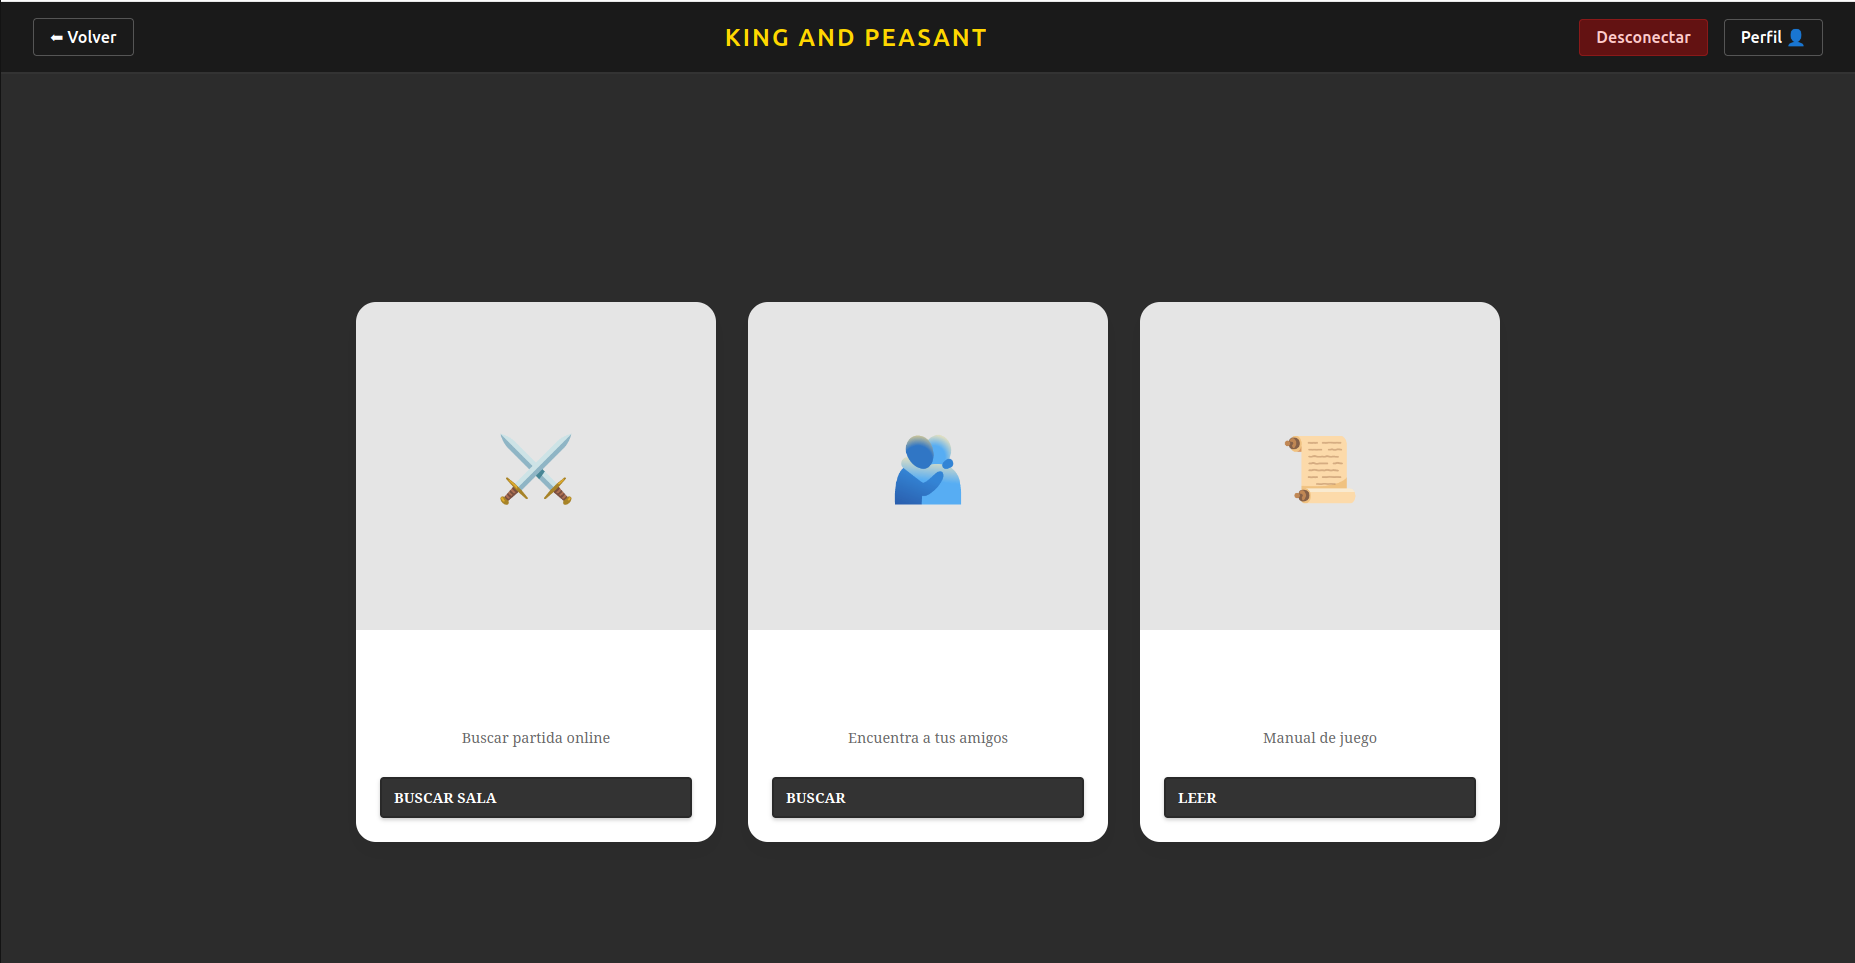
\includegraphics[width=\textwidth]{figures/manual/Pantalla Inicio.png}
\caption{Pantalla Inicio}
\label{fig:Manual01}
\end{center}
\end{figure}

Como se puede observar en la Figura \ref{fig:Manual01}, al entrar en la aplicación nos encontramos con la pantalla de inicio. Esta pantalla actúa como el eje central de navegación y presenta tres grandes paneles centrales que nos dan acceso a las distintas funcionalidades principales: ``Buscar partida online'' (para ir al listado de salas), ``Encuentra a tus amigos'' (para gestionar el aspecto social de la cuenta) y ``Manual de juego'' (para consultar las reglas).

Además, en la barra de navegación superior derecha, disponemos de botones rápidos para acceder a nuestro ``Perfil'' o para ``Desconectar'' la cuenta actual. En caso, de que no se haya iniciado sesión, aparecerán dos botones, uno para acceder al ``Registro'' y otro para acceder a la pantalla de ``Inicio de Sesión''. Para comenzar a utilizar todas estas opciones, el sistema nos requerirá haber iniciado sesión previamente.

\section{Registro/Inicio de Sesión}
\label{sec:registro}

Para acceder a las funcionalidades de la aplicación, el usuario debe identificarse. Si somos nuevos jugadores, debemos registrarnos desplegando el formulario de creación de cuenta (Figura \ref{fig:Manual02}). En este modal, titulado \textit{New Lord}, se nos solicitará introducir un nombre de usuario (\textit{Name}), un correo electrónico válido (\textit{Email}) y una contraseña segura (\textit{Password}). Tras completarlos, pulsaremos el botón rojo de \textit{Register}.

\begin{figure}[H]
\begin{center}
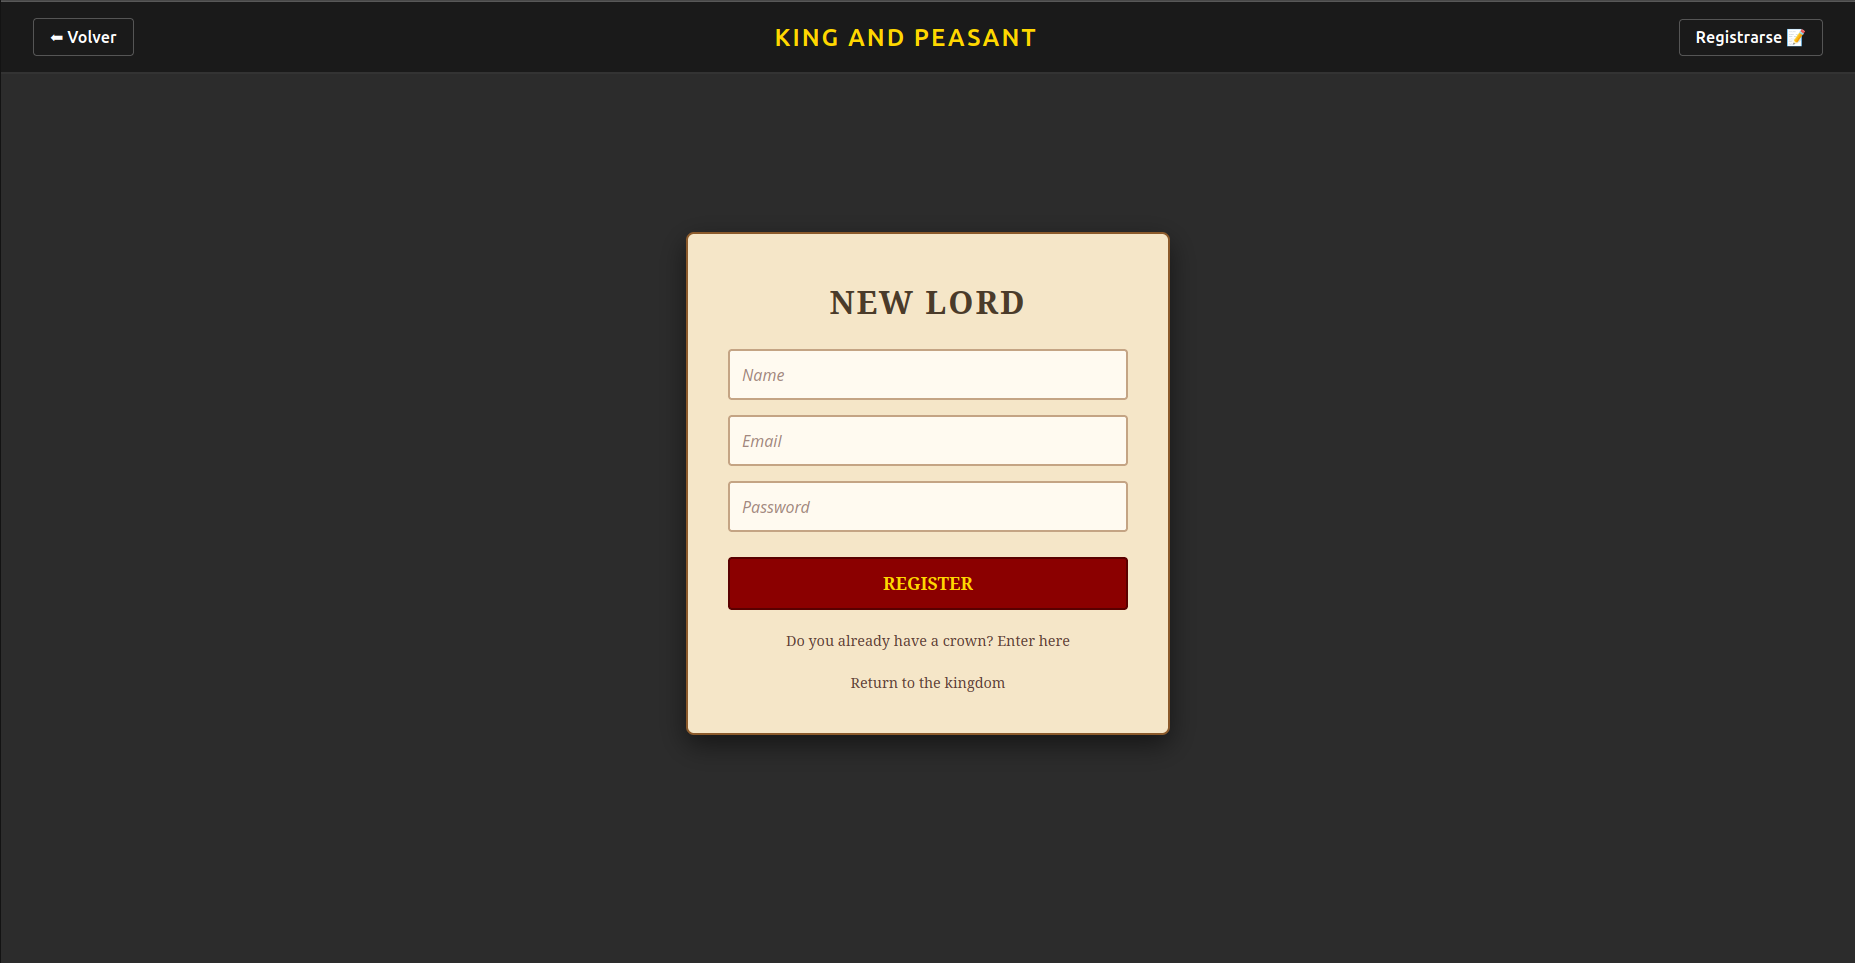
\includegraphics[width=\textwidth]{figures/manual/Registro.png}
\caption{Pantalla de Registro}
\label{fig:Manual02}
\end{center}
\end{figure}

Una vez registrados, o si ya poseíamos una cuenta previamente, podemos iniciar sesión desde la pantalla de \textit{Login} (Figura \ref{fig:Manual03}). Aquí simplemente introduciremos nuestro correo electrónico y contraseña en los campos habilitados y pulsaremos sobre el botón de confirmación. Ambas pantallas cuentan con enlaces inferiores para alternar ágilmente entre el inicio de sesión y el registro, así como para regresar a la vista principal.

\begin{figure}[H]
\begin{center}
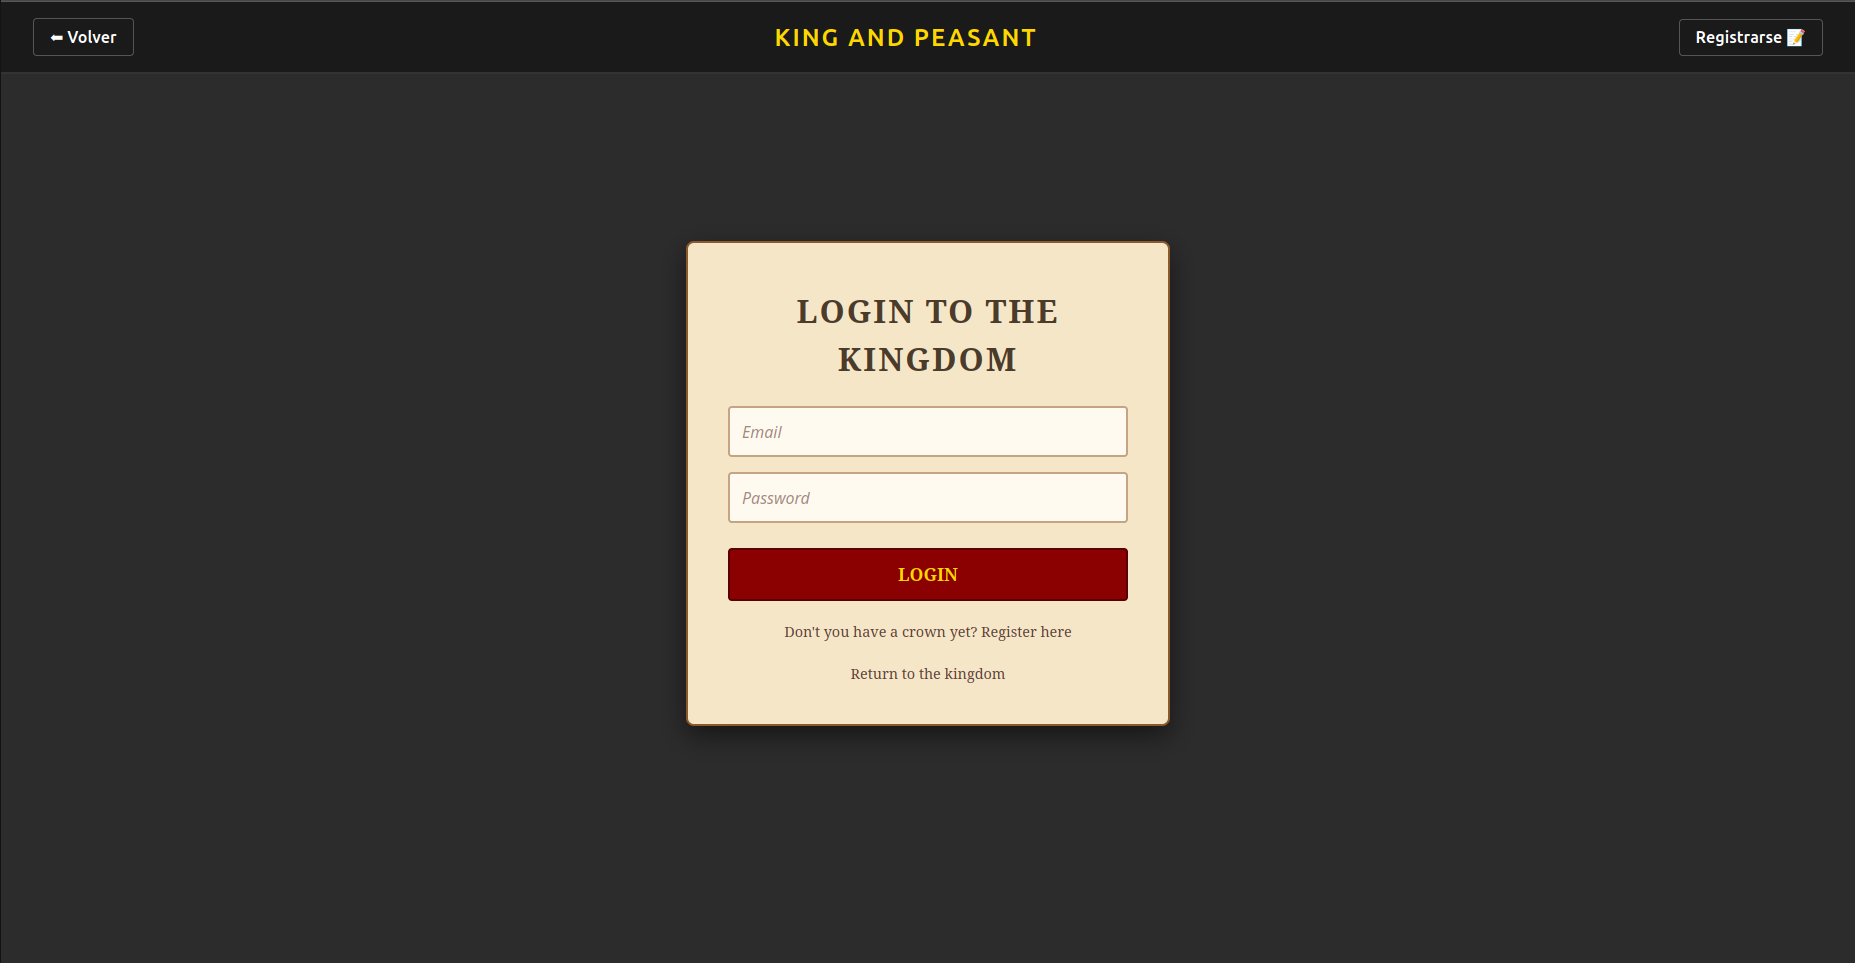
\includegraphics[width=\textwidth]{figures/manual/Login.png}
\caption{Pantalla de Inicio de Sesión}
\label{fig:Manual03}
\end{center}
\end{figure}

\section{Amistad}
\label{sec:amistad}

\begin{figure}[H]
\begin{center}
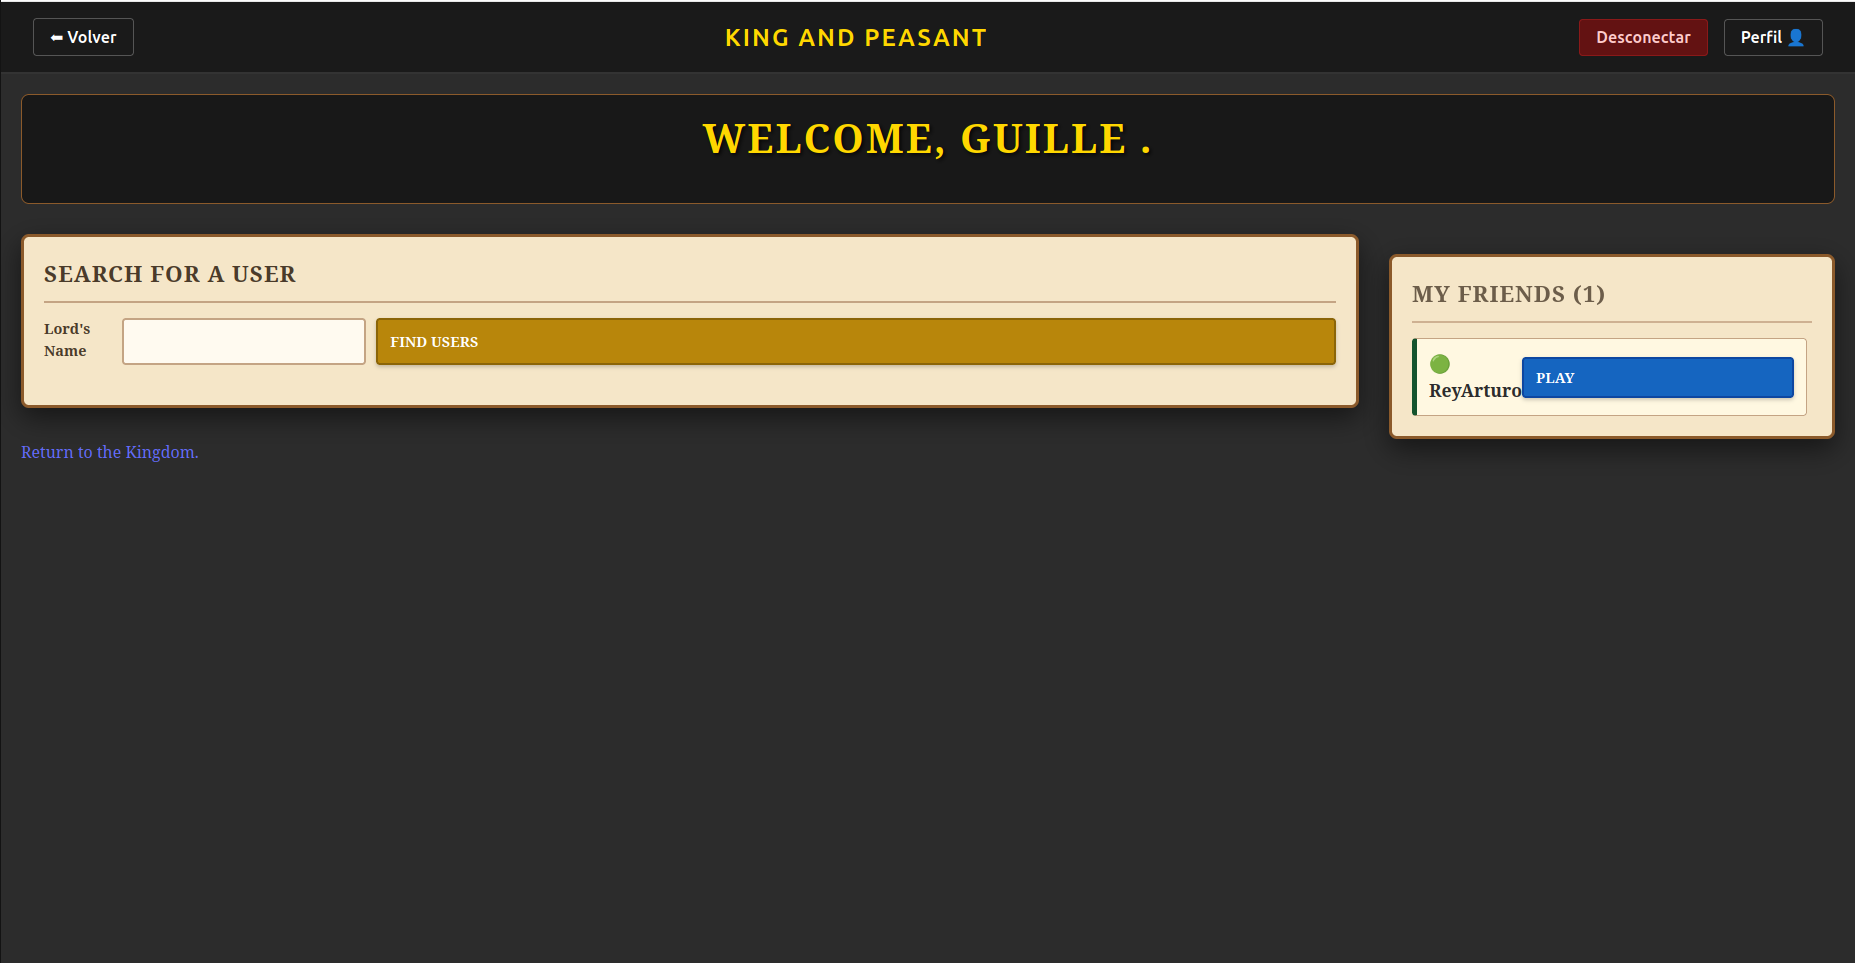
\includegraphics[width=\textwidth]{figures/manual/Amistad.png}
\caption{Pantalla de Amistad}
\label{fig:Manual10}
\end{center}
\end{figure}

La Figura \ref{fig:Manual10} ilustra la pantalla de Amistad, diseñada para la interacción con otros jugadores. La interfaz se divide en dos bloques principales. En la parte izquierda (\textit{Search for a user}), disponemos de un cuadro de texto para introducir el nombre de otro usuario y buscarlo mediante el botón \textit{Find Users}, lo que nos permite enviar nuevas peticiones de amistad.

En la parte derecha de la pantalla encontramos el panel \textit{My Friends}, que lista todos los amigos que ya tenemos agregados. Este listado muestra el nombre de cada amigo junto con un indicador visual (como un círculo verde) que señala su estado de conexión. Además, incluye un botón directo de \textit{Play} para invitar rápidamente a ese amigo a una partida sin necesidad de buscar su sala manualmente.

\section{Listado de Salas}
\label{sec:listado_salas}

\begin{figure}[H]
\begin{center}
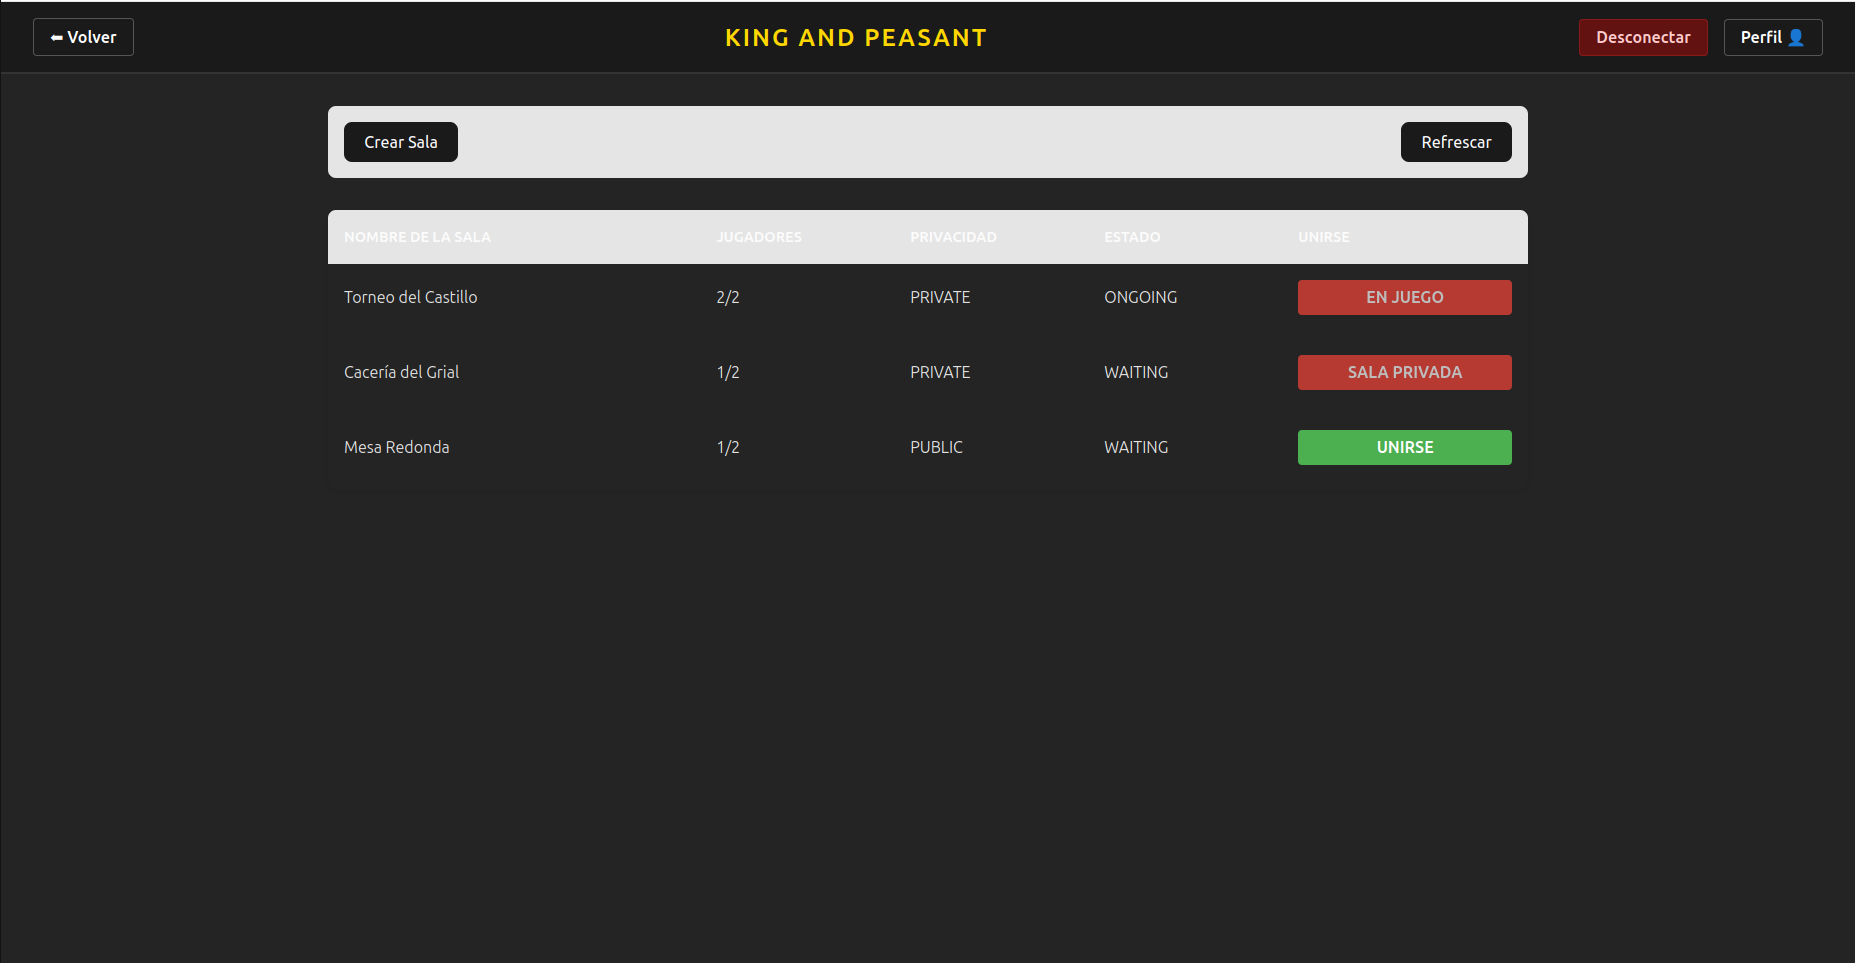
\includegraphics[width=\textwidth]{figures/manual/Listado de Salas.png}
\caption{Pantalla de Listado de Salas}
\label{fig:Manual04}
\end{center}
\end{figure}

Como se aprecia en la Figura \ref{fig:Manual04}, la pantalla de Listado de Salas presenta una tabla que recopila todas las partidas creadas en el servidor. La tabla está estructurada en cinco columnas informativas: Nombre de la Sala, Jugadores (mostrando el aforo actual frente al máximo, ej. 1/2), Privacidad (Pública o Privada), Estado (Esperando o En Juego) y una columna final de acción para Unirse. En la parte superior de la tabla contamos con un botón negro para \textit{Refrescar} la lista en tiempo real.

Desde esta interfaz podemos realizar las siguientes acciones:

\subsection{Crear Sala}

\begin{figure}[H]
\begin{center}
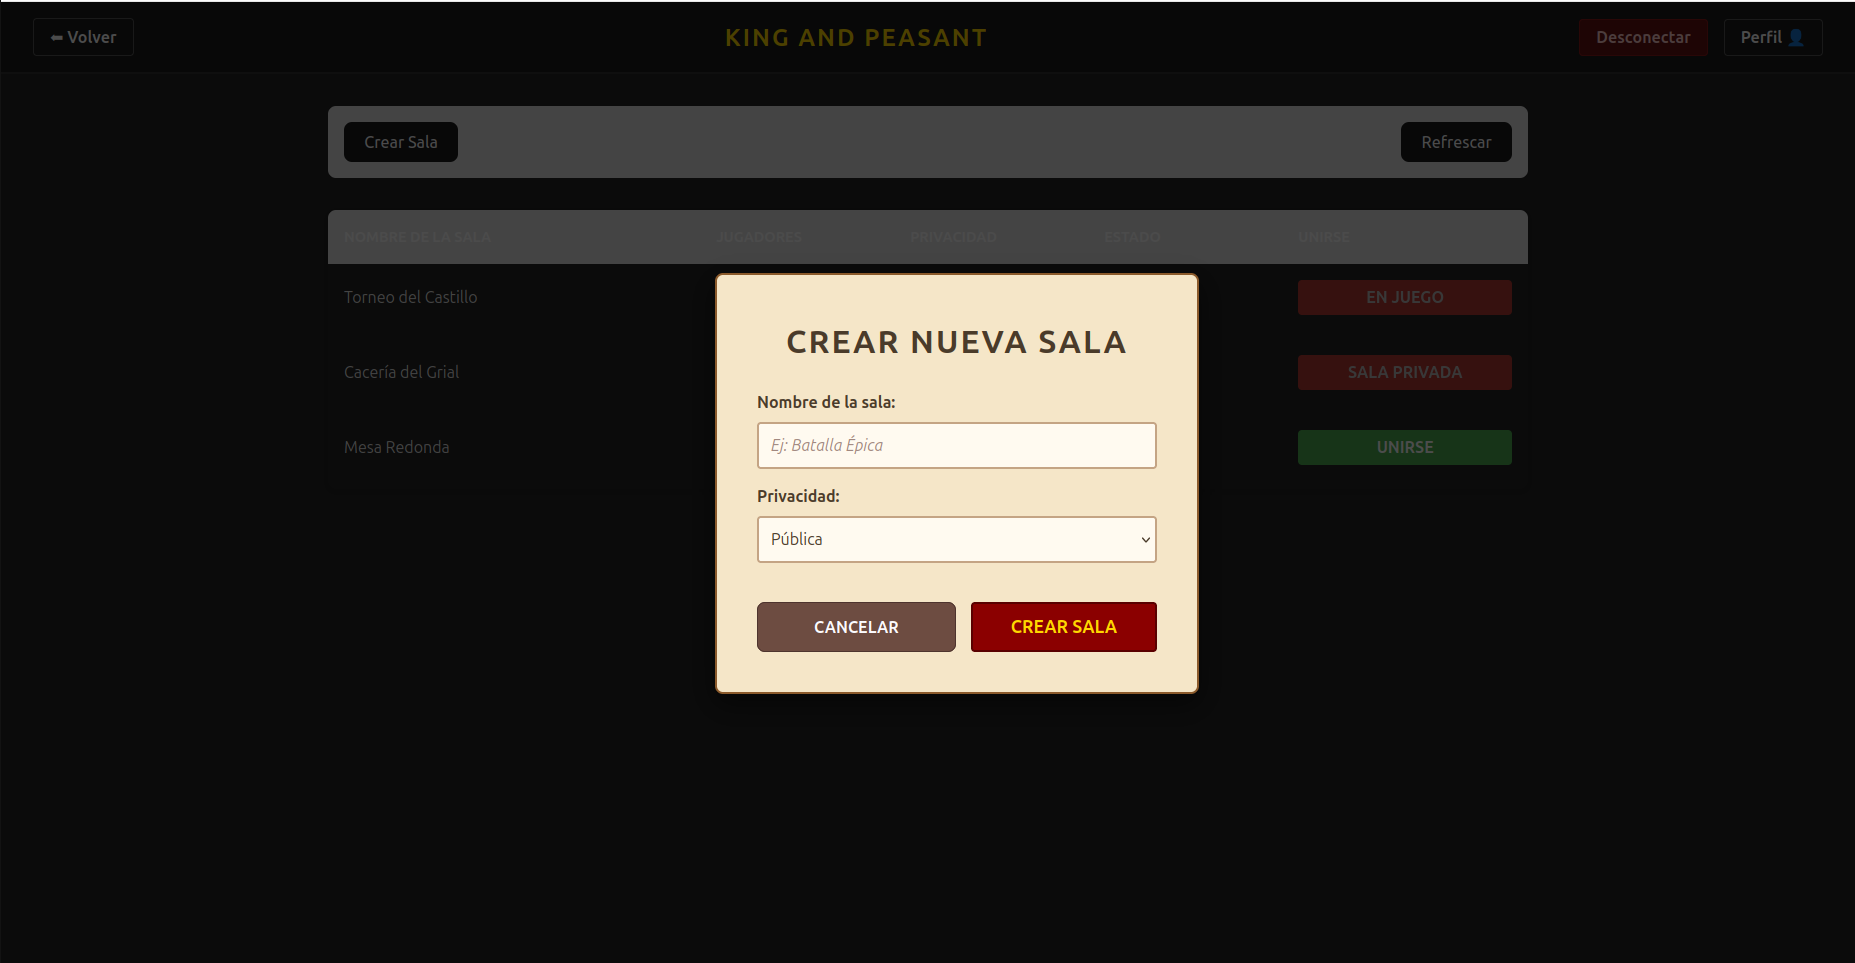
\includegraphics[width=\textwidth]{figures/manual/Crear Sala.png}
\caption{Pantalla de Listado de Salas: Crear Sala}
\label{fig:Manual05}
\end{center}
\end{figure}

Al pulsar el botón negro de \textit{Crear Sala} situado en la esquina superior izquierda, se desplegará el cuadro de diálogo mostrado en la Figura \ref{fig:Manual05}. En este formulario deberemos asignar un nombre descriptivo a nuestra sala y utilizar el menú desplegable para establecer su privacidad (determinando si cualquiera puede entrar o si requiere invitación).

\subsection{Unirse a una Sala}

Si no nos encontramos actualmente vinculados a ninguna sala, los botones de la columna derecha de la tabla estarán habilitados. Podremos pulsar el botón verde de \textit{Unirse} en aquellas salas públicas que se encuentren en estado de espera (\textit{Waiting}) y que no hayan alcanzado su límite de jugadores.

\subsection{Volver a la sala}

\begin{figure}[H]
\begin{center}
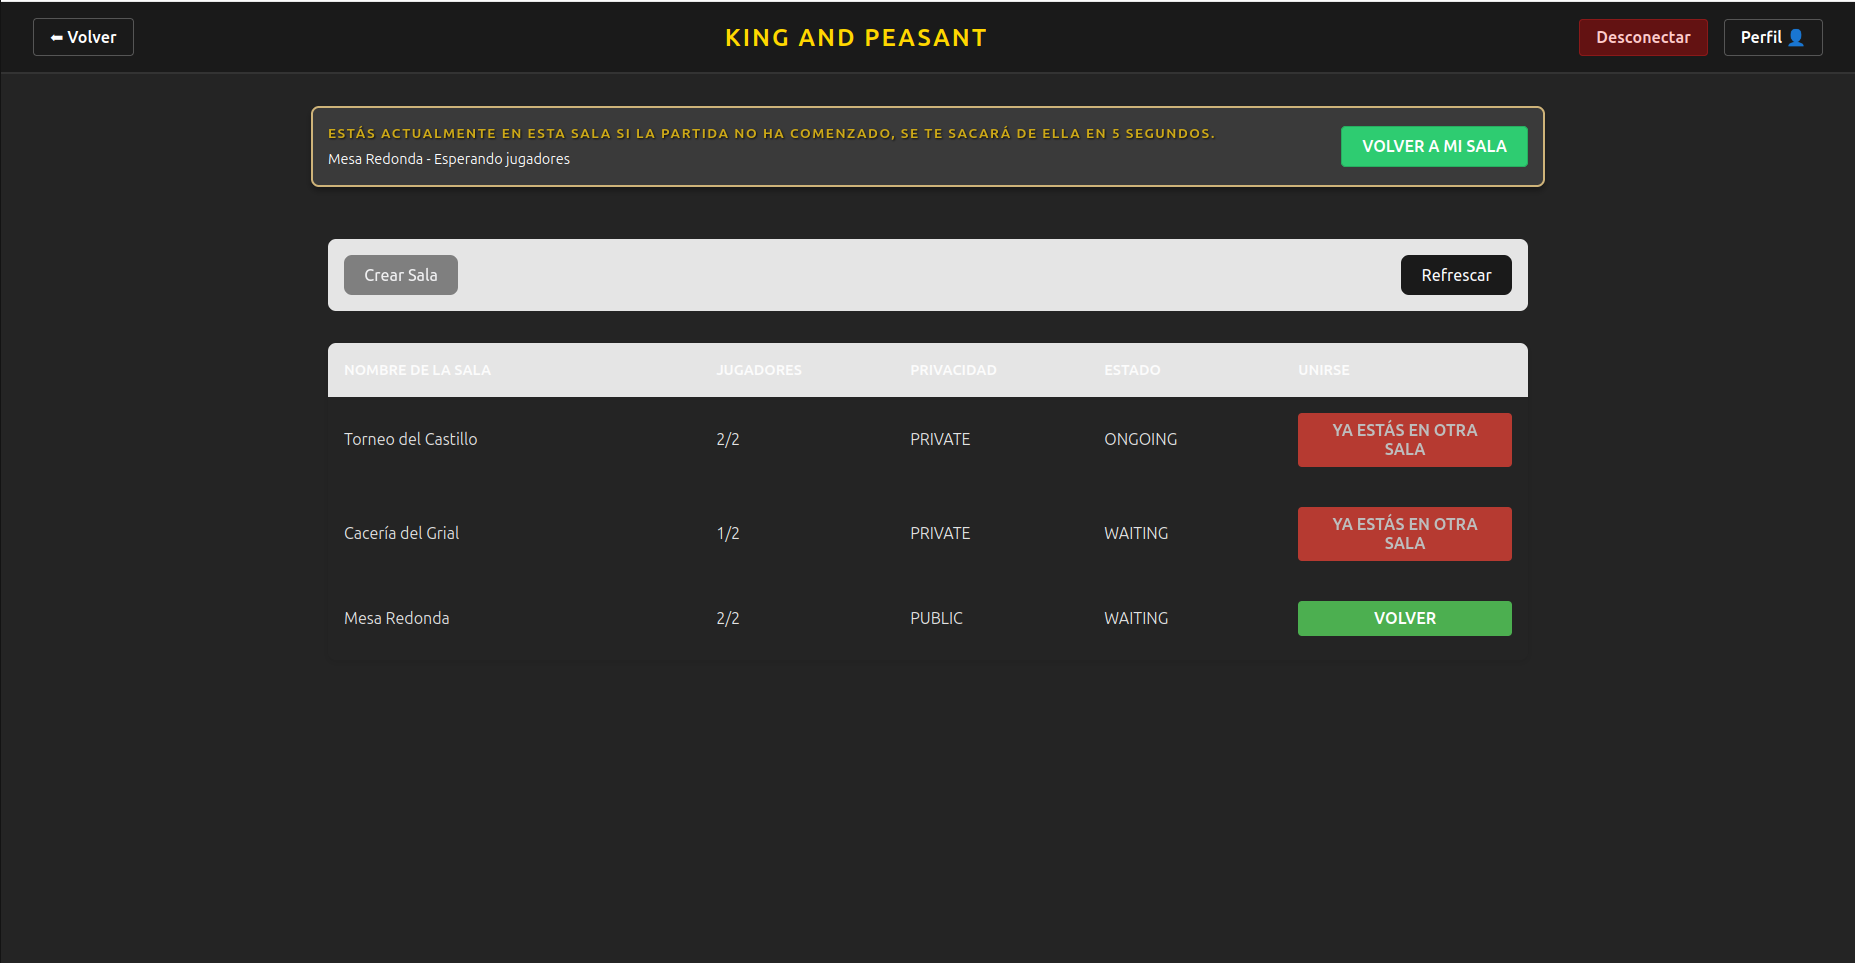
\includegraphics[width=\textwidth]{figures/manual/Volver a Sala.png}
\caption{Pantalla de Listado de Salas: Volver a la Sala}
\label{fig:Manual06}
\end{center}
\end{figure}

Tal y como detalla la Figura \ref{fig:Manual06}, si intentamos navegar por el menú mientras ya estamos dentro de una sala activa, el sistema nos alertará. Aparecerá un recuadro destacado con borde dorado en la parte superior advirtiendo que seremos expulsados de la sala en un plazo de 5 segundos si no regresamos. Para evitarlo, disponemos de un botón verde de \textit{Volver a mi sala} en ese mismo recuadro, o bien usando el botón de \textit{Volver} en la fila correspondiente de la tabla de salas.

\section{Sala}
\label{sec:sala}

\begin{figure}[H]
\begin{center}
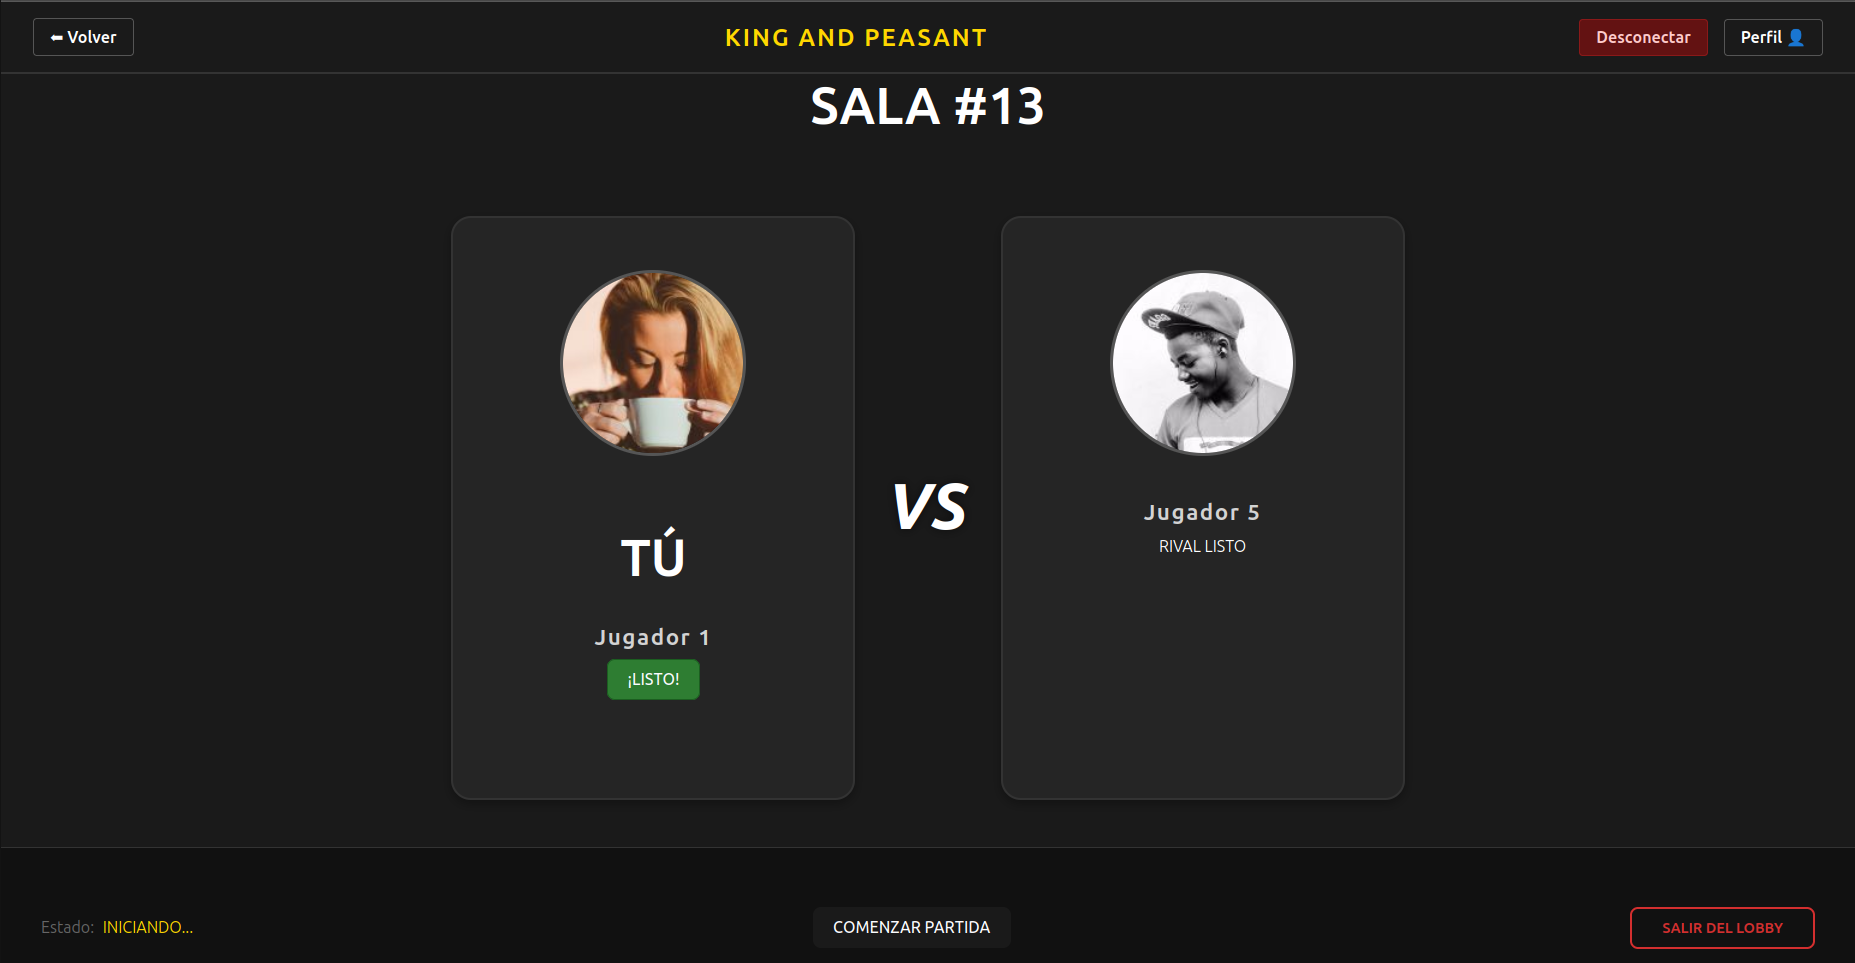
\includegraphics[width=\textwidth]{figures/manual/Sala.png}
\caption{Pantalla de Sala}
\label{fig:Manual07}
\end{center}
\end{figure}

En la Figura \ref{fig:Manual07} se expone la interfaz sala de espera previa a la partida. La pantalla muestra visualmente un enfrentamiento directo, colocando el avatar y nombre de nuestro usuario a la izquierda y los de nuestro oponente a la derecha, separados por un contundente ``VS''. 

Una vez dentro, es imperativo que marquemos el botón de \textit{¡Listo!} (ubicado bajo nuestro nombre) para confirmar nuestra disponibilidad. Cuando el sistema detecte que el texto ``Rival Listo'' aparece en el lado del oponente y nosotros también estamos preparados, el botón inferior de \textit{Comenzar Partida} se habilitará para que el creador de la sala inicie el juego. Si por algún motivo deseamos abandonar el enfrentamiento, podemos usar el botón rojo inferior derecho de \textit{Salir del Lobby}, lo que nos devolverá al listado de salas.

\section{Partida}
\label{sec:partida}

\subsection{Interfaz del Juego}
\begin{description}
    \item \textbf{Tu Área:}

    \begin{figure}[H]
    \begin{center}
    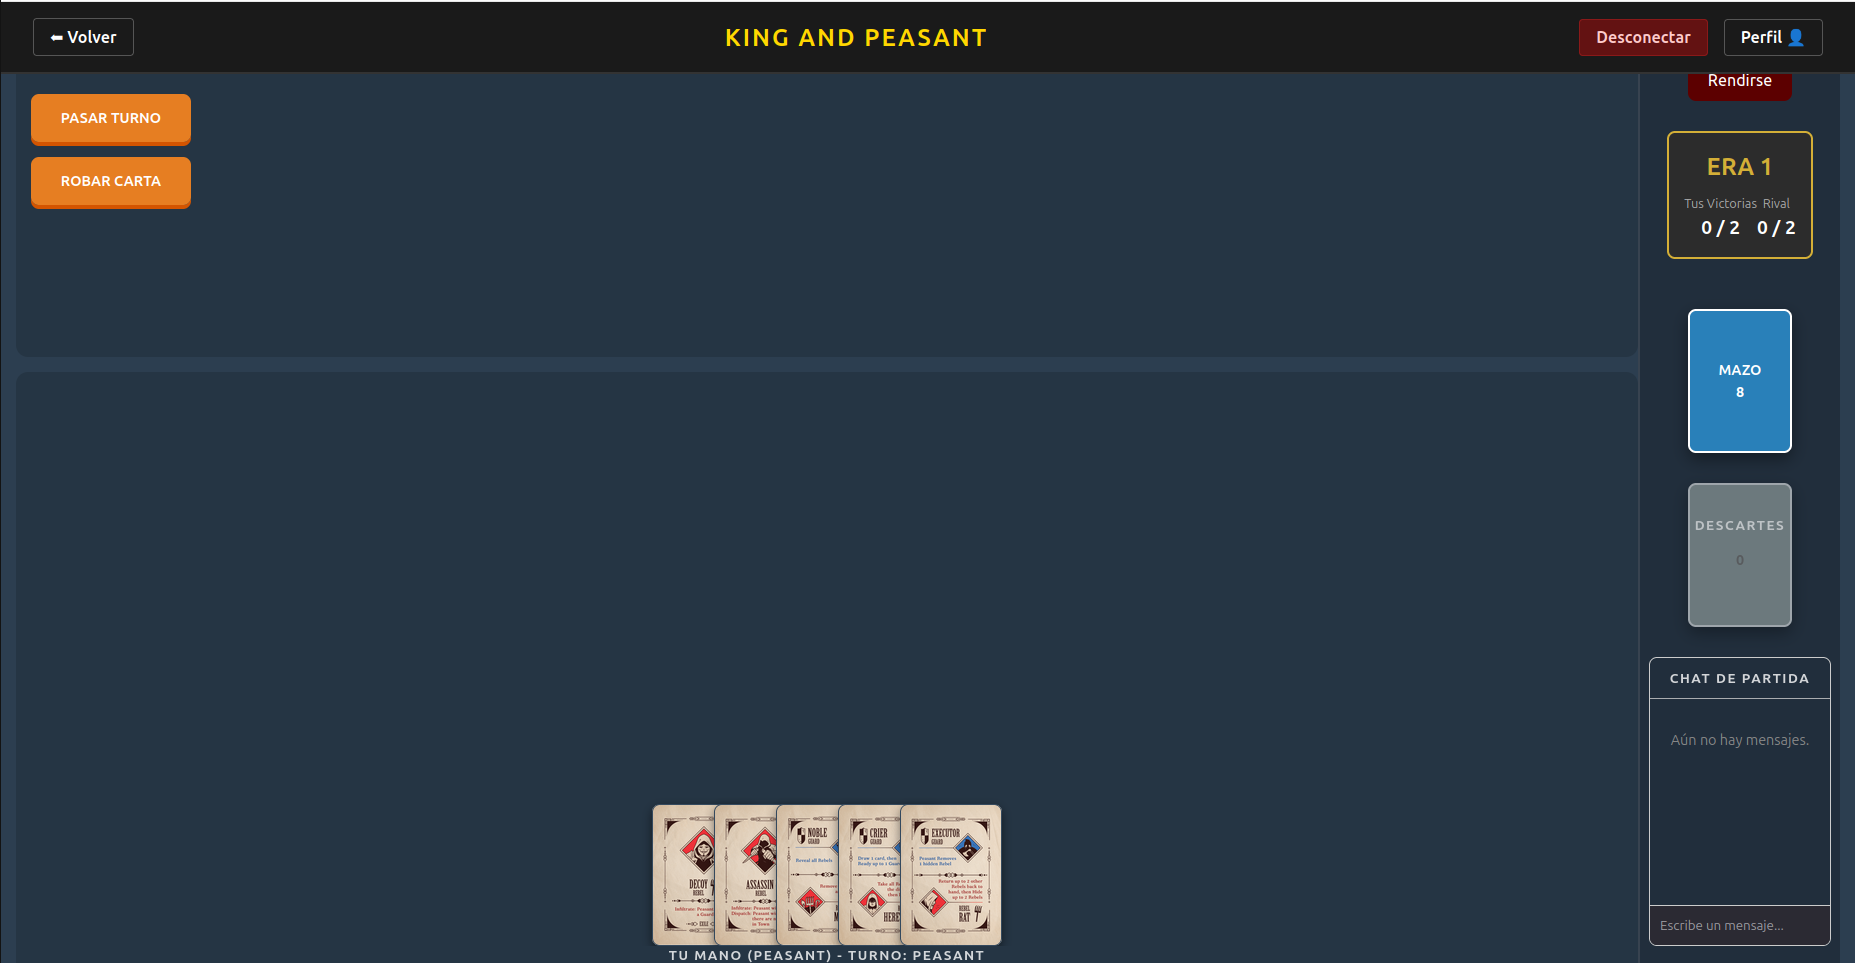
\includegraphics[width=\textwidth]{figures/manual/Partida Tu Mano.png}
    \caption{Pantalla de Partida: Tu Área}
    \label{fig:Manual08}
    \end{center}
    \end{figure}

    La Figura \ref{fig:Manual08} muestra la perspectiva inferior del tablero correspondiente a nuestro control. En la parte central inferior se despliegan boca arriba las cartas que conforman nuestra mano actual. Justo debajo de ellas, un indicador de texto nos recuerda en todo momento nuestro rol y de quién es el turno (por ejemplo: \textit{Tu mano (Peasant) - Turno: Peasant}). Sobre nuestra mano se extiende nuestro territorio del pueblo, la zona designada para colocar estratégicamente nuestras unidades durante el desarrollo del juego. 

    \item \textbf{Área del Rival:}

    \begin{figure}[H]
    \begin{center}
    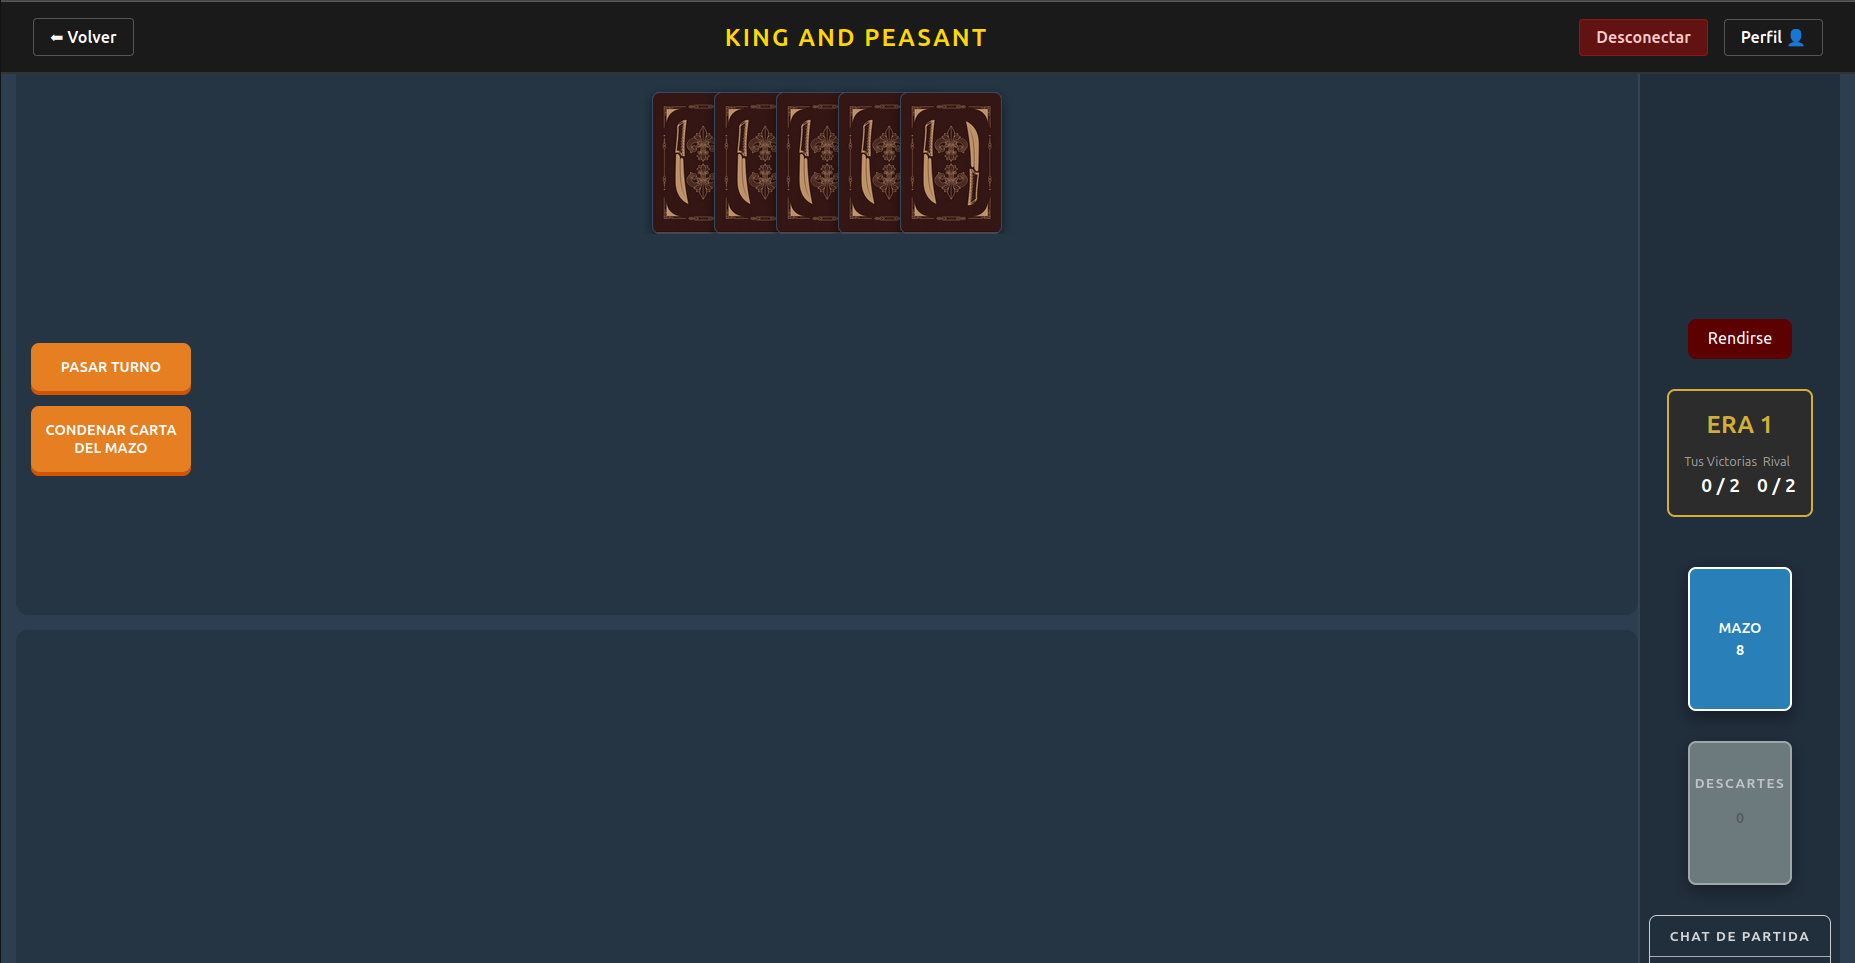
\includegraphics[width=\textwidth]{figures/manual/Partida Mano Rival.png}
    \caption{Pantalla de Partida: Área del Rival}
    \label{fig:Manual09}
    \end{center}
    \end{figure}

    En la Figura \ref{fig:Manual09} se ilustra la mitad superior de la pantalla, dedicada al oponente. En el extremo superior se visualizan las cartas de su mano, las cuales permanecen boca abajo revelando únicamente su reverso. Bajo su mano se encuentra el territorio del pueblo rival. Las cartas que el adversario coloque aquí se mostrarán boca abajo si están ocultas, o boca arriba si han sido reveladas como consecuencia de las acciones de la partida.

    \item \textbf{Panel Lateral Izquierdo (Acciones):}
    
    A la izquierda del tablero principal (visibles en color naranja) se ubican los botones de acción rápida, cuyo contenido varía en función del turno y la situación. Acciones habituales como \textit{Pasar Turno}, \textit{Robar Carta} o \textit{Condenar Carta del Mazo} aparecerán en esta columna para ser ejecutadas ágilmente.

    \item \textbf{Panel Lateral Derecho (Estado y Comunicación):}
    
    En la franja derecha se agrupa la información global de la partida. Arriba encontramos un botón rojo para \textit{Rendirse}, seguido de un marcador que indica la ronda actual (\textit{Era 1}) y el conteo de victorias de ambos jugadores. Debajo de esto se sitúan dos botones grandes: el mazo principal en color azul (indicando cuántas cartas restan por robar) y la pila de descartes en color gris. En la zona inferior derecha disponemos de una caja de chat en vivo para comunicarnos con nuestro rival.
\end{description}

\subsection{Acciones de Turno}

Durante tu turno, podrás interactuar con la interfaz para realizar diversas acciones dependiendo de tu rol estratégico (Rey o Campesino) y del estado del tablero:

\begin{description}

    \item \textbf{Robar Carta:}

    Pulsando el botón naranja correspondiente en el menú izquierdo, extraerás la primera carta del mazo para añadirla a tu mano.

    \item \textbf{Colocar Carta en Pueblo:}

    Haciendo clic sobre una carta de tipo \texttt{Guard} o \texttt{Rebel} en tu mano, la trasladarás a tu zona del pueblo en el tablero.

    \item \textbf{Jugar Carta en el Pueblo:}

    Selecciona una carta del pueblo para jugar su acción. En caso de que tu rol sea el de Campesino, solo puedes jugar cartas no reveladas.

    Si la carta se puede infiltrar, deberás seleccionarla y elegir la posición del mazo de forma interactiva donde quieres infiltrar la carta.

    \item \textbf{Jugar Acción:}

    Si seleccionas una carta de tipo \texttt{ACTION} directamente desde tu mano, su efecto se aplicará de inmediato y la carta irá a los descartes, sin necesidad de transitar previamente por el pueblo.

    \item \textbf{Pasar Turno:}

    Utilizando el botón naranja de \textit{Pasar Turno} ubicado en la columna izquierda, finalizarás tus acciones y cederás el control al adversario.

    \item \textbf{Condenar Rebelde:}

    Si juegas bajo el rol del Rey, la interfaz te habilitará la opción letal de condenar a un rebelde no revelado. Puedes ejecutar esto haciendo clic directo sobre una carta oculta en el pueblo rival, o usando el botón \textit{Condenar Carta del Mazo} del panel izquierdo para ejecutar la carta superior del mazo. 

    \texttt{CUIDADO: Esta acción es definitiva. Culminará inmediatamente en victoria o derrota para el Rey dependiendo de si la carta ejecutada resulta ser el Asesino.}

    \item \textbf{Acciones Pendientes:}

    El flujo normal del juego puede verse interrumpido cuando una carta jugada por tu rival requiera tu intervención obligatoria (por ejemplo, seleccionar un objetivo válido). La interfaz central te exigirá tomar una decisión y seleccionar una respuesta válida antes de permitirte continuar con otras acciones.
\end{description}

\section{Fin de la Era y Fin de la Partida}
\label{sec:fin_partida}

Una vez que se cumplen las condiciones de victoria específicas de alguno de los dos roles, el tablero se bloquea y aparece una pantalla modal anunciando al ganador de la ronda actual. Este cuadro ofrece un resumen estadístico rápido de la Era finalizada y contiene un botón de confirmación que ambos jugadores deben pulsar para proceder a la siguiente ronda.

El sistema lleva el registro acumulativo en el panel lateral. En el momento en que un jugador logre alzarse con la victoria en dos Eras distintas, el juego declarará el final definitivo de la partida y la interfaz redirigirá automáticamente a ambos usuarios de vuelta a la sala de espera original.

%!TEX root =  tfg.tex
\chapter{Conclusiones}

\begin{abstract}
Este capítulo presenta una evaluación final del Trabajo Fin de Grado y del proceso de desarrollo de \textit{King and Peasant}. El objetivo es realizar una reflexión crítica sobre los resultados obtenidos, analizando tanto los aciertos técnicos y organizativos como las dificultades encontradas a lo largo del ciclo de vida del proyecto. Finalmente, se expondrán las posibles líneas de investigación y desarrollo que podrían dar continuidad a este trabajo en el futuro.
\end{abstract}

\section{Informe post-mortem}

El informe post-mortem constituye un ejercicio de retrospectiva fundamental en la ingeniería de software. Su propósito no es únicamente evaluar el producto final, sino analizar el proceso de desarrollo en su conjunto, identificando las prácticas que han aportado valor y aquellas áreas donde la planificación o ejecución no fueron óptimas. Esto permite extraer lecciones aprendidas aplicables a futuros proyectos en un entorno profesional.

\subsection{Lo que ha ido bien}

\begin{itemize}
\item \textbf{Arquitectura y sincronización en tiempo real:} La integración de \textit{WebSockets} junto con Node.js y React ha demostrado ser un acierto absoluto. Se ha logrado una comunicación bidireccional fluida que mantiene la integridad del motor de reglas y proporciona la inmediatez requerida en un entorno multijugador asimétrico.

\item \textbf{Trabajo en equipo y sinergia:} El desarrollo conjunto ha permitido abordar un proyecto de gran envergadura dividiendo la carga de forma eficaz. La colaboración activa y la comunicación constante han facilitado la resolución de problemas técnicos complejos y la implementación integral de las mecánicas del juego, demostrando la viabilidad y las ventajas del trabajo en equipo.

\item \textbf{Metodología de trabajo y control de calidad:} La adopción de un enfoque iterativo propio ha resultado muy favorable. Además, el hecho de estipular un periodo de pruebas exclusivo e independiente en el calendario de planificación, en lugar de realizar testeos fragmentados por cada tarea, permitió concentrar los esfuerzos de validación de forma eficiente y asegurar la estabilidad global del sistema.
\end{itemize}

\subsection{Lo que ha ido mal}

\begin{itemize}
\item \textbf{Iteraciones sin descansos:} La planificación inicial no contempló intervalos de descanso estructurados (ya fuesen días libres dentro de las iteraciones o semanas de pausa entre las mismas). La exigencia del desarrollo continuo y sin pausas provocó una fatiga acumulada que, en determinados momentos, se tradujo en una bajada de la moral y del rendimiento general del equipo.

\item \textbf{Gestión de estados asíncronos complejos:} La traducción de las reglas del juego de mesa físico al motor digital resultó más laboriosa de lo estimado. La gestión de estados concurrentes y las validaciones estables en el servidor generaron ciertos cuellos de botella técnicos durante las primeras fases de implementación de la partida.

\item \textbf{Curva de aprendizaje inicial:} Aunque el resultado final es robusto, el dominio inicial de la programación orientada a eventos para el correcto flujo del patrón Modelo-Vista-Controlador (MVC) en tiempo real supuso un desafío temporal que ajustó los márgenes de desarrollo.
\end{itemize}

\subsection{Discusión}

En función de lo anterior, si el proyecto comenzara hoy de nuevo, el principal cambio a nivel técnico radicaría en el diseño inicial de la arquitectura de eventos del servidor. Se invertiría más tiempo en una fase de diseño para estandarizar los mensajes entre cliente y servidor antes de comenzar la implementación del código. Por otro lado, a nivel organizativo, se modificaría drásticamente la planificación del calendario para incluir pausas y periodos de descanso obligatorios entre iteraciones, garantizando así un ritmo de trabajo más sostenible que preserve la motivación, la salud mental y la productividad a lo largo de todo el ciclo de vida del software.

\section{Trabajos futuros}

El desarrollo de \textit{King and Peasant} ha establecido una base técnica sólida y escalable, pero existen diversas funcionalidades que, por viabilidad y delimitación del alcance, quedaron fuera del sistema actual. Entre los puntos abiertos destacan:

\begin{itemize}
    \item \textbf{Sistema competitivo (\textit{Ranked}) y Matchmaking:} Implementación de un sistema de emparejamiento basado en habilidades y puntuaciones de clasificación global (tipo Elo).
    \item \textbf{Inteligencia Artificial (PvE):} Desarrollo de agentes autónomos que permitan a los usuarios jugar partidas en solitario para practicar estrategias sin necesidad de un rival humano.
    \item \textbf{Desarrollo móvil nativo y Monetización:} Adaptación del entorno web a aplicaciones dedicadas para iOS y Android para captar un público más amplio, e integración de una economía virtual o pasarelas de pago.
\end{itemize}

Estas características darían lugar a una expansión natural del proyecto actual. Se podría acotar como el desarrollo de una versión 2.0 de la plataforma orientada a la fidelización de usuarios a largo plazo y la competición, tomando la actual arquitectura contenerizada, el sistema de perfiles y el motor de reglas base como el núcleo inalterable sobre el que construir y acoplar los nuevos microservicios.




\part{Appendices}
\appendix

\chapter{Manual Oficial de King and Peasant}
\label{anexo:reglas_juego}

% El parámetro pages=- le dice que incluya TODAS las páginas del PDF.
% pagecommand={} hace que se mantenga la numeración de páginas de tu TFG.
% width=\textwidth ajusta el PDF a los márgenes de tu memoria.
\includepdf[pages=-, width=\textwidth, pagecommand={}]{figures/reglas_del_juego.pdf}

\input{ejemplo}

\lineNumbersOff

\setglossarystyle{long}
\printglossaries
\newpage

\bibliographystyle{abbrvnat}
\addcontentsline{toc}{chapter}{Referencias bibliográficas}
\bibliography{referencias}

\end{document} 